\documentclass[10pt, conference, compsocconf]{IEEEtran}

\usepackage{graphics}
\usepackage[pdftex]{graphicx}
\graphicspath{{figures/}}
\usepackage[cmex10]{amsmath}
%\usepackage{amsmath}
%\usepackage{amssymb}
\usepackage{amsfonts}
\usepackage{fixltx2e}
\usepackage{url}
% \usepackage[colorlinks,linkcolor=blue,urlcolor=blue,citecolor=blue]{hyperref}
\usepackage[nocompress]{cite}
% correct bad hyphenation here
\hyphenation{op-tical net-works semi-conduc-tor}

% Include other packages here, before hyperref.

% If you comment hyperref and then uncomment it, you should delete
% egpaper.aux before re-running latex.  (Or just hit 'q' on the first latex
% run, let it finish, and you should be clear).
%\usepackage[pagebackref=true,breaklinks=true,letterpaper=true,colorlinks,bookmarks=false]{hyperref}

\newcommand{\Eq}[1] {Eq.~(\ref{eq:#1})}
\newcommand{\Fig}[1]{Fig.~\ref{fig:#1}}
\newcommand{\Sec}[1]{Sec.~\ref{sec:#1}}
\newcommand{\Eqs}   {Eqs.~}
\newcommand{\Figs}  {Figs.~}
\newcommand{\Tbl}[1]{Table~\ref{tbl:#1}}
\newcommand{\Etal}  {{\it et al.}}
\newcommand{\Figa}[1]{Fig.~\ref{fig:#1}(a)}
\newcommand{\Figb}[1]{Fig.~\ref{fig:#1}(b)}
\newcommand{\Figc}[1]{Fig.~\ref{fig:#1}(c)}
\newcommand{\Figd}[1]{Fig.~\ref{fig:#1}(d)}



% *** Do not adjust lengths that control margins, column widths, etc. ***
% *** Do not use packages that alter fonts (such as pslatex).         ***
% There should be no need to do such things with IEEEtran.cls V1.6 and later.
% (Unless specifically asked to do so by the journal or conference you plan
% to submit to, of course. )


% correct bad hyphenation here
%\hyphenation{op-tical net-works semi-conduc-tor}


\begin{document}
%
% paper title
% can use linebreaks \\ within to get better formatting as desired
\title{\Large\bf Lightweight 3D Modeling of Urban Buildings From Range Data}

\author{\IEEEauthorblockN{Weihong Li}
\IEEEauthorblockA{Department of Computer Science\\
Graduate Center, City University of New York\\
New York, USA\\
wli@gc.cuny.edu}
\and
\IEEEauthorblockN{George Wolberg}
\IEEEauthorblockA{Department of Computer Science\\
City College of New York\\
New York, USA\\
wolberg@cs.ccny.cuny.edu}
\and
\IEEEauthorblockN{Siavash Zokai}
\IEEEauthorblockA{Brainstorm Technology LLC\\
New York, USA\\
zokai@brainstorm.com}
}


% make the title area
\maketitle

%%%%%%%%% ABSTRACT
\begin{abstract}
Laser range scanners are widely used to acquire accurate scene measurements.
The massive point clouds they generate, however, present challenges to
efficient modeling and visualization.
State-of-the-art techniques for generating 3D models from voluminous
range data is well-known to demand large computational and storage requirements.
In this paper, attention is directed to the modeling of urban buildings
directly from range data.
We present an efficient modeling algorithm that exploits \emph{a priori}
knowledge that buildings can be modeled from cross-sectional contours
using extrusion and tapering operations.
Inspired by this simple workflow, we identify key cross-sectional slices among
the point cloud.
These slices capture changes across the building facade along the principal axes.
Standard image processing algorithms are used to remove noise, fill missing
data, and vectorize the projected points into planar contours.
Applying extrusion and tapering operations to these contours
permits us to achieve dramatic geometry compression, making the resulting
models suitable for web-based applications such as Google Earth
or Microsoft Virtual Earth.
This work has applications in architecture, urban design, virtual city
touring, and online gaming.
We present experimental results on synthetic and real urban building
datasets to validate the proposed algorithm.
\end{abstract}

\vskip 0.5em
%\begin{IEEEkeywords}
{\bf {\emph{Keywords}} -  3D Modeling, point cloud, laser scanning, range data, segmentation, Google SketchUp, vectorization
}
%\end{IEEEkeywords}


%%%%%%%%% BODY TEXT
\section{Introduction}

The 3D modeling of urban buildings is an area of active research
with increasing attention drawn from the computer graphics and
computer vision communities.
Current state-of-the-art algorithms include procedural modeling,
3D laser scanning, and image-based approaches.
In addition, conventional modeling tools are commonly used for this purpose.
The most accurate input source for modeling {\it existing} buildings, though,
remains laser range scanners.
They provide high geometric detail by collecting range data from hundreds
of meters away with an accuracy on the order of a few millimeters.
This fidelity is appropriate for construction, architecture, cultural
heritage, and forensics applications.
Unfortunately, laser range scanning can produce an overwhelming amount of data,
which poses great challenges to visualization software that require lightweight
3D models for interactive use.
Polygonal data generated from range scans are therefore too dense for use in
web-based applications such as Google Earth and Microsoft Virtual Earth.
These applications work best with lightweight models consisting of only
hundreds of polygons.

The goal of this work is to automatically produce high-quality
lightweight models of urban buildings from large-scale 3D range data.
The proposed solution is inspired by the simple paradigm embedded in
procedural modeling as well as interactive tools such as Google SketchUp.
A key idea is that a simple set of extrusion and tapering
operations applied to 2D contours can grow a wide array of complex 3D urban
models.
We propose a reverse engineering approach to infer key cross-sectional
planar contours along with a set of extrusion and tapering operations to derive
lightweight models that conform to the 3D range data.

The proposed algorithm can generate models across a wide spectrum of
resolutions.
A particularly useful feature of the algorithm is that it outperforms
existing approximation techniques by preserving the sharpness of the raw
data, even at low resolution.
The contribution of this work is that it combines the benefits of
\emph{a priori} knowledge of urban buildings and fast 2D image
processing techniques to perform 3D modeling of urban buildings directly
from point cloud data (PCD).
This offers the benefit of a cost-effective geometry compression
approach for voluminous range data within the domain of urban structures.
It can be applied to boost web-based 3D applications, virtual city touring,
and online gaming.

\section{Related Work}

\begin{figure*}[htbp]
\begin{center}
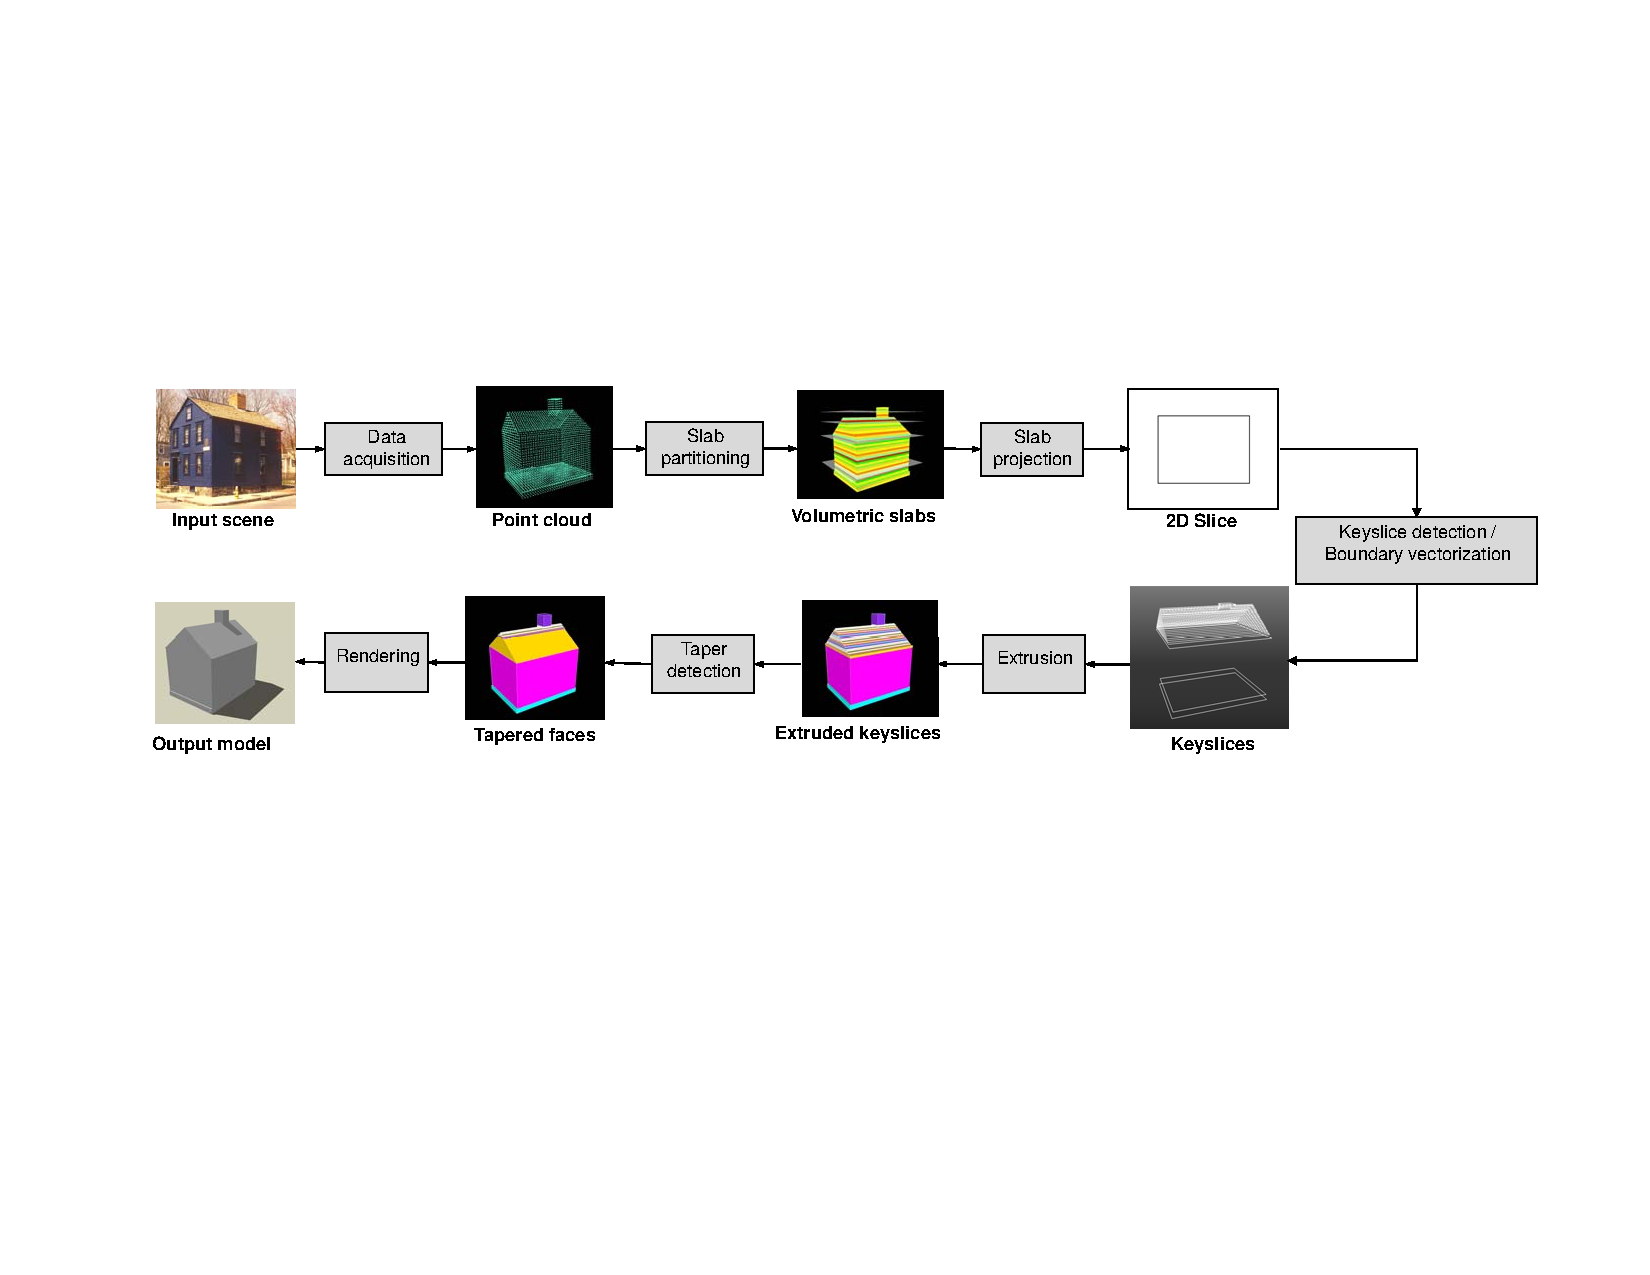
\includegraphics[width=7in]{overview.pdf}
\end{center}
%\vspace{-0.2in}
\caption{Overview of the proposed approach.}
\label{fig:ov}
\end{figure*}

In an attempt to steer clear of tedious and expensive hand-made models,
procedural modeling of buildings in \cite{PMB_MWH} has been proposed.
By using an effective description language, buildings and streets of a virtual
city can be generated automatically.
The strength of this approach is that the description language can generate
a huge number of buildings and streets quickly and beautifully.
This is particularly useful for gaming and other computer graphics applications.
However, since the parameters used to generate the buildings are randomly
generated, the city generated with these buildings and streets is a virtual one.
This approach is not useful for attempting to model an {\it existing} building.
To do so, one has to manually specify the parameters of the building,
which is very cumbersome.
Our goal is to automatically infer the contours and parameters
of an existing building directly from dense range data.

Reconstruction of 3D models from range data has been addressed in
\cite{RE_Fisher} with applications in numerous research areas,
including computer-aided design (CAD), computer vision, architectural modeling,
and medical image processing.
The authors in \cite{Okorn10} use a histogram of height data to detect floors
and ceilings for creating accurate floor plan models of building interiors.
In \cite{DP_OWYC}, the authors proposed a 3D building reconstruction from a
2D floorplan image.
With the help of a 2D floorplan image, both the interior and exterior of a
building can be reconstructed accordingly.
A survey on methods for generating 3D building models from architectural
floor plans is given in \cite{YIN09}.
However, reliance on 2D floor plans makes this approach too limiting for
most applications, including our project.

In \cite{RE_TOGSH}, known manufacturing features were used to infer the
3D structure of mechanical parts.
Their method benefits from the domain knowledge that most of the mechanical
parts consist of predefined structures, such as holes, bosses, and grooves.
Our work is partially motivated by this idea since it also incorporates
{\it a priori} knowledge about the construction of urban buildings for further
inference.
However, their method is based on predefined simple geometry structures and
the assumption that the input 3D data has no holes.
This hinders their approach for applications with incomplete data.

Multimodal data fusion is another approach for large-scale urban
environment modeling.
In \cite{UM_Zakhor}, both air and ground data are fused, including
laser scans, camera images, and aerial images.
The LIDAR scans are used to create the models and the camera images are used
for texture mapping.
Citing the cumbersome and expensive use of laser scanners, the researchers
in \cite{AKBARZADEH06} propose an approach that relies solely on passive
sensors (cameras) mounted on a moving vehicle.
Dense 3D point cloud measurements are derived using their multiview stereo
module based on multiple plane sweeping directions.
In an attempt to compress the voluminous data produced in the method of
\cite{AKBARZADEH06}, Xiao et al. \cite{UM_XFTQ} introduced an alternate
approach for modeling facades along a street using prior knowledge about
the buildings.
They achieve geometry compression and deliver a clean approximation of the
facades by applying a combination of plane fitting and window detection.
Their method, however, relies on limited assumptions about the planarity of
the buildings.
The method introduced in this paper, however, places no such limitations.
We can handle facades of any shape that exploit extrusion and tapering operations.
Toshev {\it et al.} proposed a grammar based method for detecting and parsing
buildings from unorganized street-level point clouds \cite{RW_TMT} .
Despite its efficiency in modeling, the results could not generate
enough level of details for the buildings.

In \cite{luo08}, the authors divide the point cloud into slices from which
circles can be fitted to extract pillars of buildings.
Although we also use slices of point cloud data, our work generalizes to
arbitrary profiles and multiple sweeping directions.
In related work, \cite{gonzalvez07} uses 2D slices of point cloud data
to segment simple primitives such as lines and arcs.
Clustering these 2D primitives from slice to slice is used to fit
planes and cylinders to the 3D data.
This limits the work to recovering only simple planar and cylindrical fragments
of the complete model.
The remaining segments are left as point cloud data.

%%%%%%%%%%%%%%%%%%%%%%%%%%%%%%%%
%%%%%%   Overview  %%%%%%%%
%%%%%%%%%%%%%%%%%%%%%%%%%%%%%%%%
\section{Overview}

We propose an efficient way to reconstruct 3D models from range data by
partitioning the data into thin cross-sectional volumetric slabs.
For each slab, all range data in that slab is projected onto a 2D
cross-sectional contour slice.
Producing this array of slices permits us to avoid costly computation directly
on 3D data.
A similarity measure is used to cluster the sliced images
together into {\it keyslices}.
This term is analogous to the use of ``keyframes'' in computer animation,
which denote important snapshots in the animation sequence from which
intermediate results can be derived.
In essence, each keyframe is a slice in the spatiotemporal volume of
an animation.
Similarly, each keyslice is a 2D image which contains a {\it transitional}
cross-section of the building, encapsulating major contours in the facade.
The model is then generated by applying basic extrusion and tapering
operations from one keyslice to the next.
This produces a lightweight representation consisting of only a few
hundred polygons.

\begin{figure} [htbp]
\begin{center}
\begin{tabular}{c}
\fbox{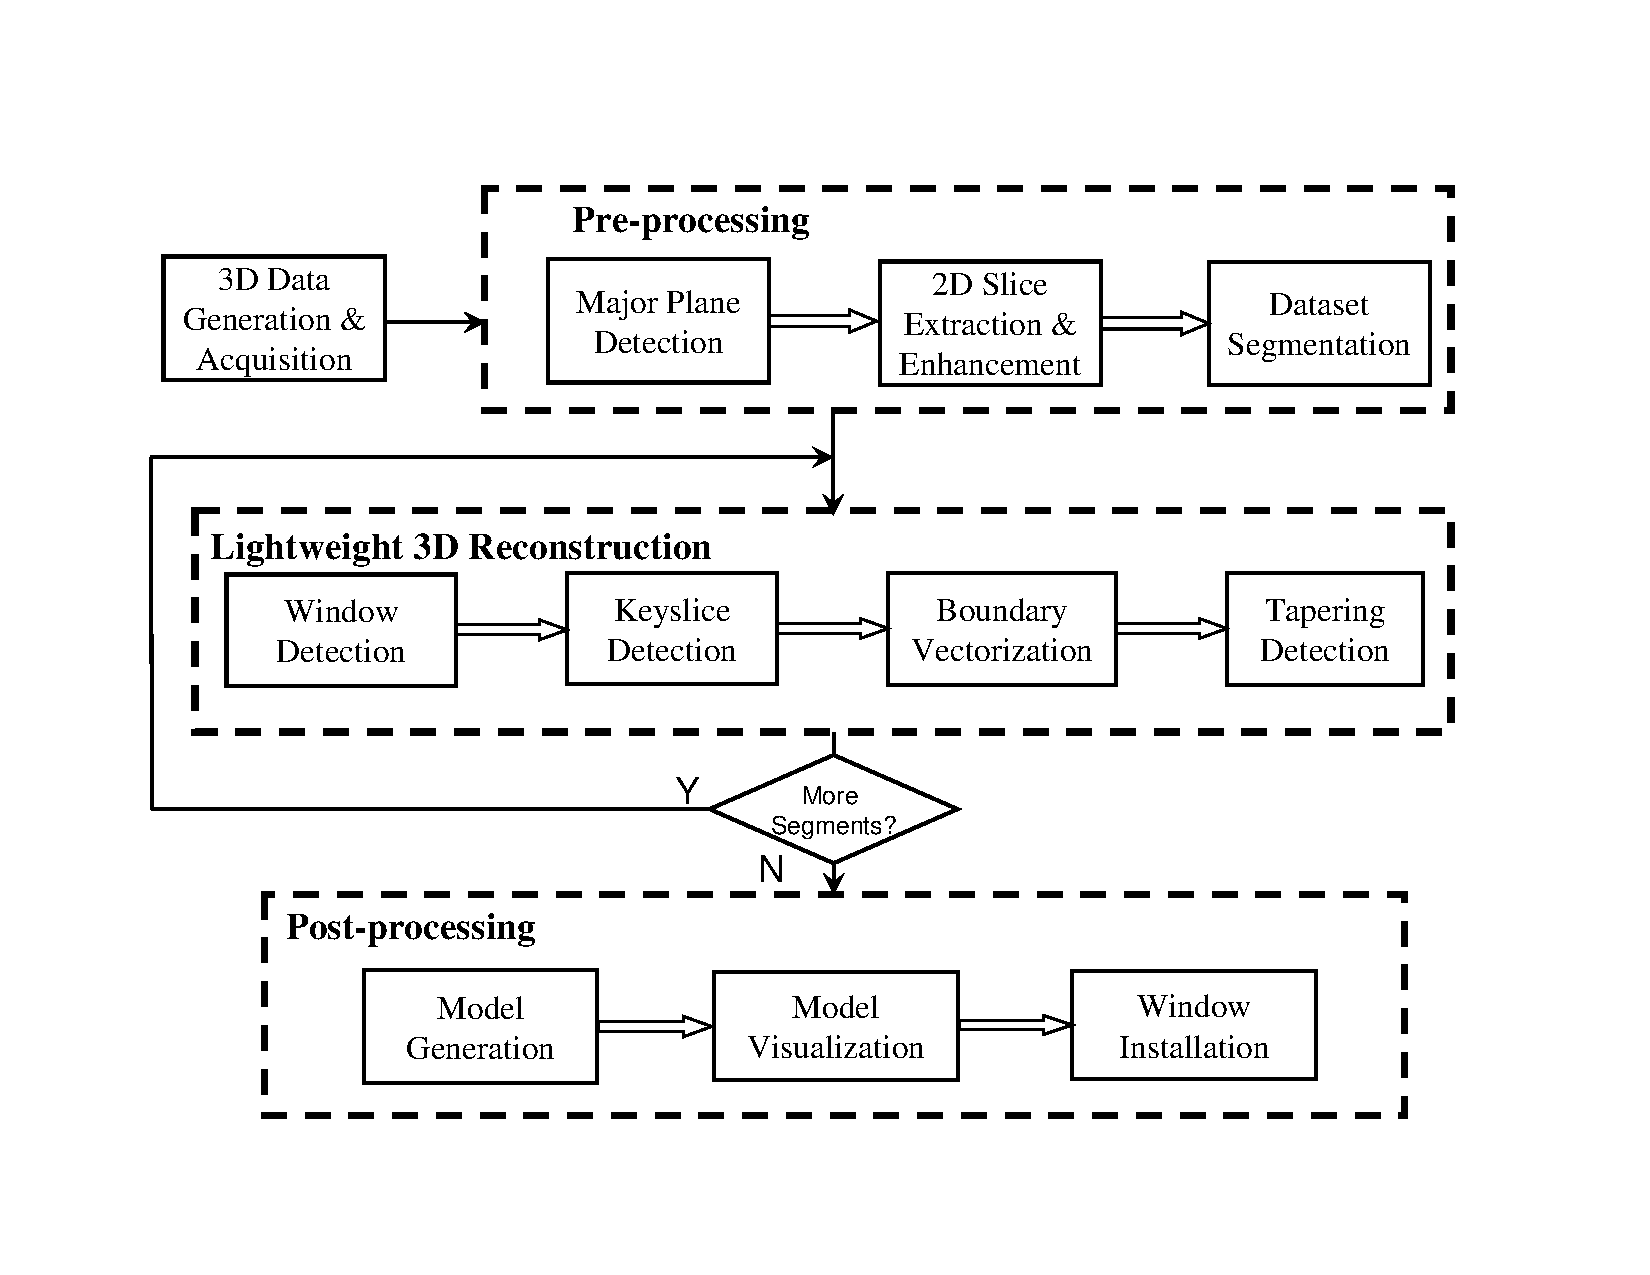
\includegraphics[width=0.45\textwidth]{flow.pdf}}
\end{tabular}
\end{center}
\caption{
The flow diagram of the system.
}
\label{fig:flow}
\end{figure}

\Fig{ov} depicts the basic concept of our algorithm.
We begin with the
acquisition of a dense 3D point cloud $C$ of a building.
$C$ is then partitioned into a nonoverlapping set of volumetric slabs.
Each slab $S$ is associated with one projection plane $P$,
sitting at the base of $S$.
The purpose of partitioning $C$ is to establish a set of cross-sections,
or contour slices.
By examining the changes among these slices, we can identify the prominent
slices, or {\it keyslices}, as well as the necessary extrusion and
tapering operations that must apply to them to generate the model.
By casting this 3D modeling task into a series of 2D operations, we
reduce the dimension of the problem to achieve a significant savings in
computational complexity.

The modular flow diagram for our system is shown in \Fig{flow}.
The whole system consists of three stages of computation.
In the first pre-processing stage,
2D slices are extracted from the heavy 3D range data and
are enhanced by noise removal and the filling of missing data.
The segmentation module is then carried out to divide the complicated
3D dataset into simpler segments.
The second stage is iteratively applied to each segment,
including window detection, keyslice detection, boundary vectorization,
and tapering detection.
The final stage reconstructs each segment and assembles them into a whole model.

%%%%%%%%%%%%%%%%%%%%%%%%%%%%%%%%
%%%%%%   PREPROCESSING  %%%%%%%%
%%%%%%%%%%%%%%%%%%%%%%%%%%%%%%%%
\section{Preprocessing the Range Data}
\label{sec:prep}

The input to our system is range data assembled as a 3D point cloud.
%The basic algorithm that we use for registering the voluminous 3D data
%acquired from multiple scans of buildings has been introduced in
%\cite{RDP_LS}.
We have registered the voluminous 3D data acquired from multiple scans of buildings
using the algorithm in \cite{Stamos08}.
That same algorithm is also responsible for extracting the major axes
of the building in order to align it to the axes of the world coordinate
system.
This is necessary to properly infer the keyslices.
\Figb{IR_2_DXF} displays a properly aligned, {\it registered} 3D point cloud.

\begin{figure}[htbp]
\begin{center}
\begin{tabular}{cc}
	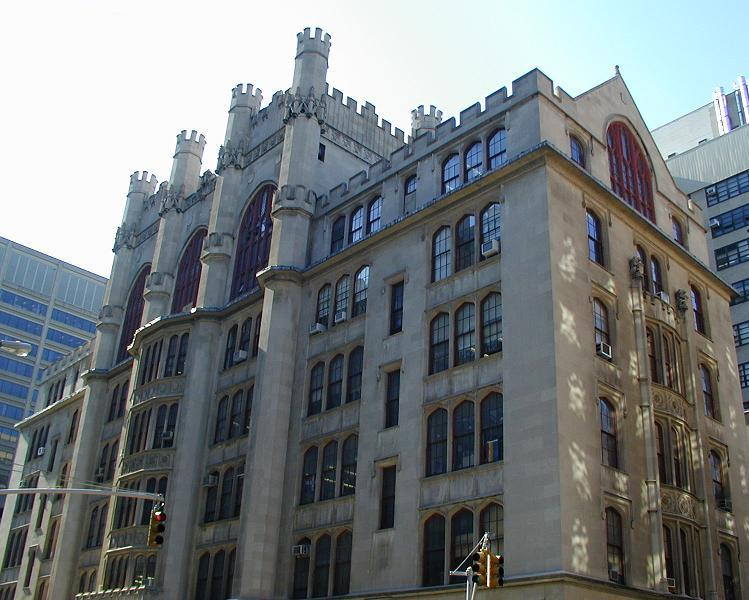
\includegraphics[width=0.22\textwidth]{HunterPhoto.jpg} &
	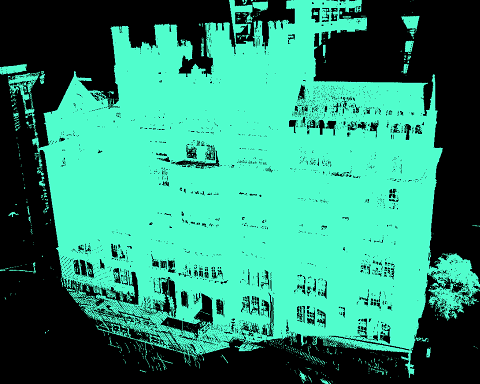
\includegraphics[width=0.22\textwidth]{point_cloud.png} \\
	(a) & (b) \\
\end{tabular}
\end{center}
\caption{
(a) Input scene.
(b) 3D point cloud of scene assembled by registering 14 scans, each having
one million points.
}
\label{fig:IR_2_DXF}
\end{figure}

In addition to real data, we also generated some synthetic datasets for experiments.
These synthetic datasets were sampled from 3D building models
containing 3D faces and their normals,
which were downloaded from Google 3D warehouse.
The first two rows of \Fig{results} show two such models and their 3D point
clouds in (a) and (b), respectively.

\subsection{Major Plane Detection}
\label{sec:major_plane}

The input to our system consists of unorganized 3D point clouds.
We solve for the major planes, whose normals are the sweeping directions
from which to extract 2D slices.
These slices are the starting point for segmentation and window detection.
We used moving least squares (MLS) for deriving a smooth plane from a set
of neighboring data points in space for normal computation.
After the normal is computed for each 3D point, the Hough transform was used
to identify the major plane normals based on voting \cite{MLS01}.
These normals will determine the orientation of the cross-sections that
sweep through the PCD.

\subsection{Extraction of 2D Slices}
\label{sec:image_slicing}

We consider the PCD as a large array of 3D points to be
sliced into equispaced parallel volumetric slabs.
All 3D points within each slab are projected onto a projection plane, or slice,
at the base of the slab.
\Figa{slice_slab} shows the 3D point cloud in \Figb{IR_2_DXF} partitioned into
50 slabs.
The projected 3D points in each slab form cross-sectional contour slices.
\Fig{slicing} depicts four such slices, associated with the four displayed
projection planes of \Figa{slice_slab}.

\begin{figure} [htbp]
\begin{center}
\begin{tabular}{cc}
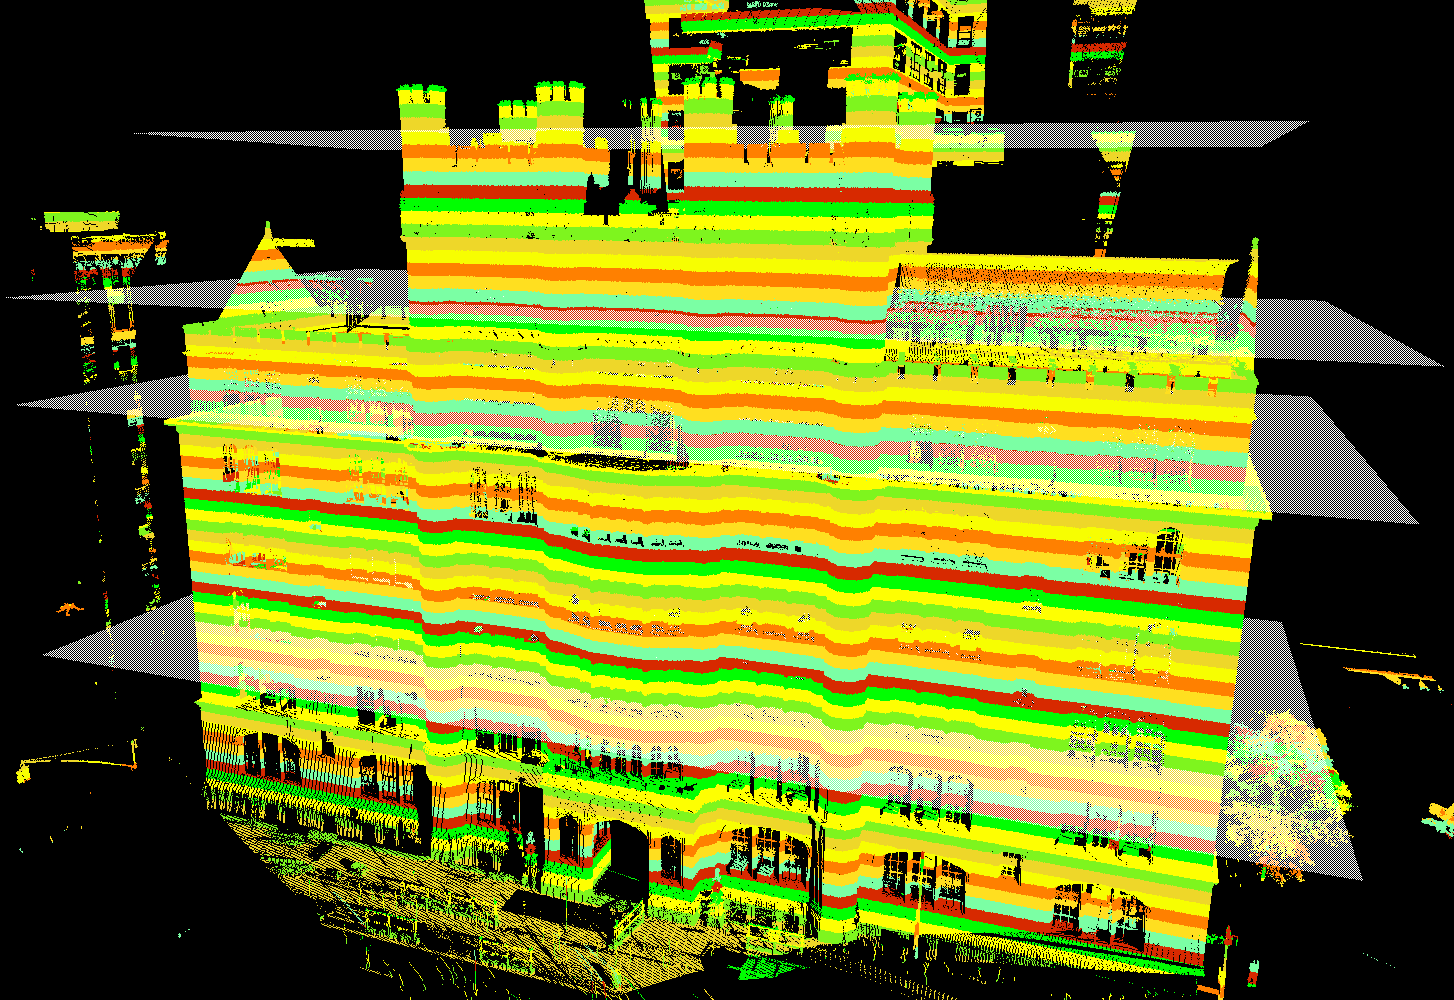
\includegraphics[width=0.22\textwidth]{slab_planar.png} &
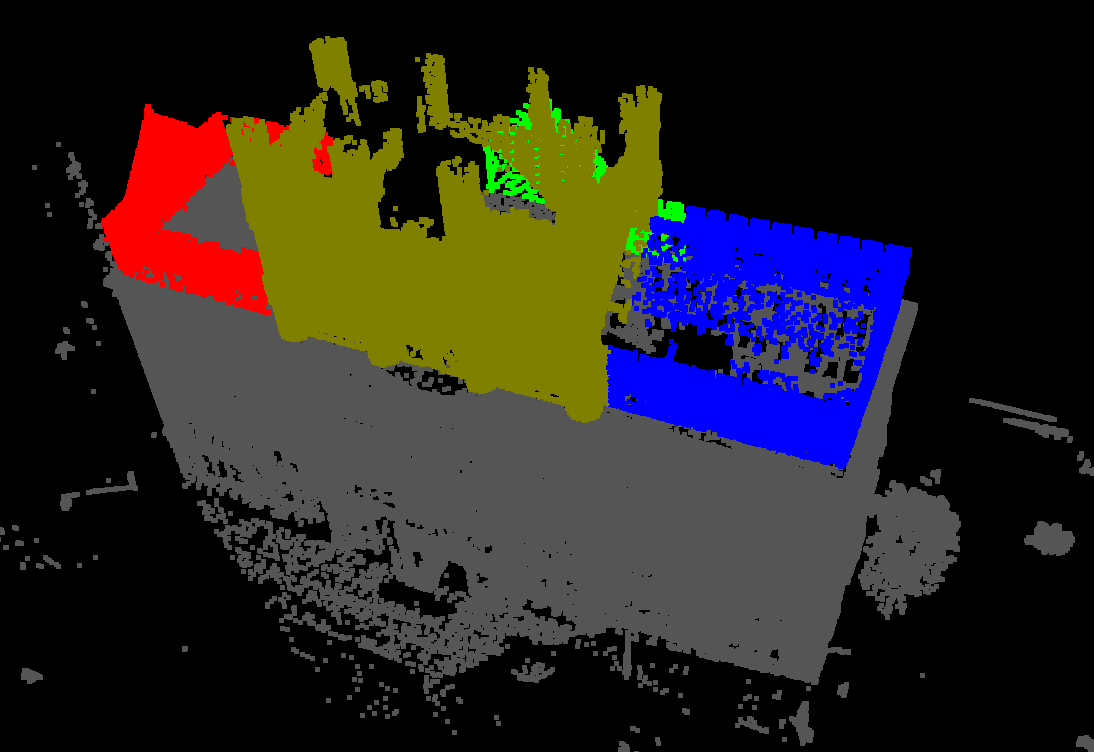
\includegraphics[width=0.22\textwidth]{TH_7_crop.png}
\end{tabular}
\end{center}
\caption{(a) The 3D point cloud of \Figb{IR_2_DXF} partitioned into uniform
volumetric slabs.
The 3D points in each slab are projected onto a projection plane to
form cross-sectional slices. Four such planes are shown;
(b) Segmentation result of \Figb{IR_2_DXF}.}
\label{fig:slice_slab}
\end{figure}

%The height of each slab is $\boldsymbol{\delta}$.
%If $\boldsymbol{\delta}$ is held constant, each slice is generated from
%equi-spaced slab intervals.
%If $\boldsymbol{\delta}$ is allowed to vary, then we may
%choose to allow for large values in parts of the structure that are similar,
%and low values in regions that contain finer detail.

\begin{figure} [htbp]
\begin{center}
\begin{tabular}{cc}
\fbox{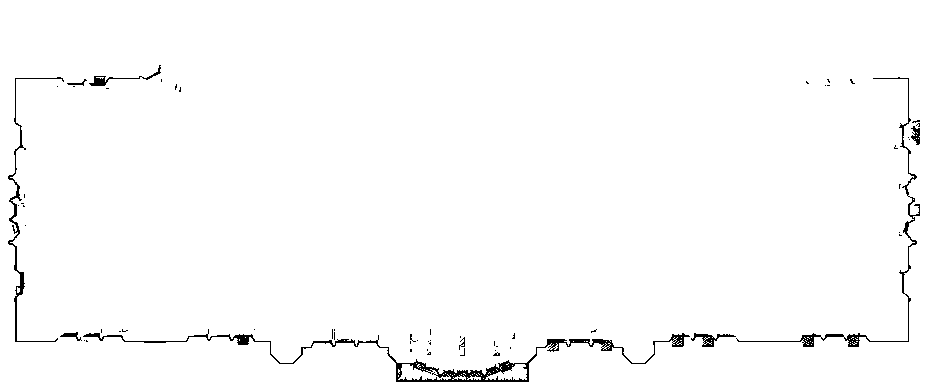
\includegraphics[width=0.2\textwidth]{image_slice_0190.png}} &
\fbox{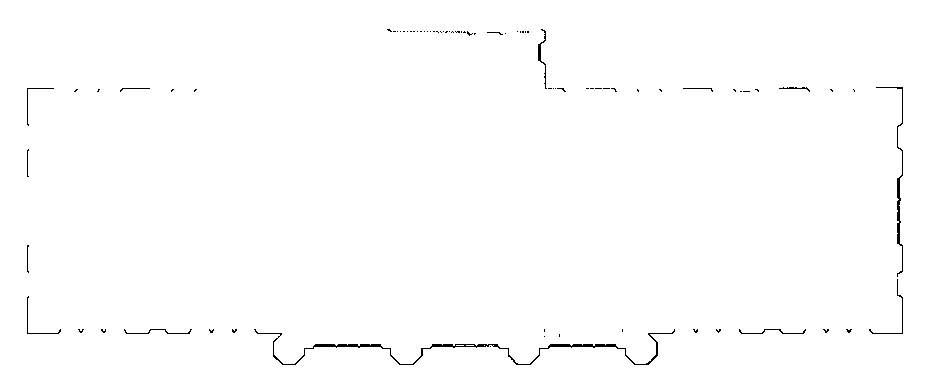
\includegraphics[width=0.2\textwidth]{image_slice_0600.png}} \\
(a) & (b) \\
\fbox{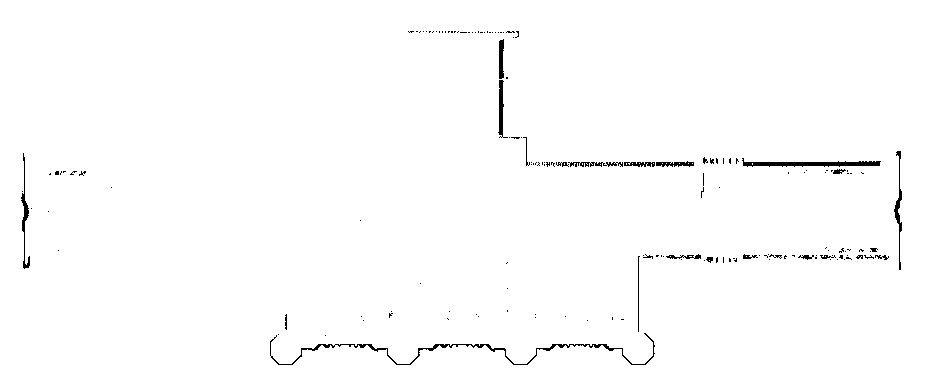
\includegraphics[width=0.2\textwidth]{image_slice_0714.png}} &
\fbox{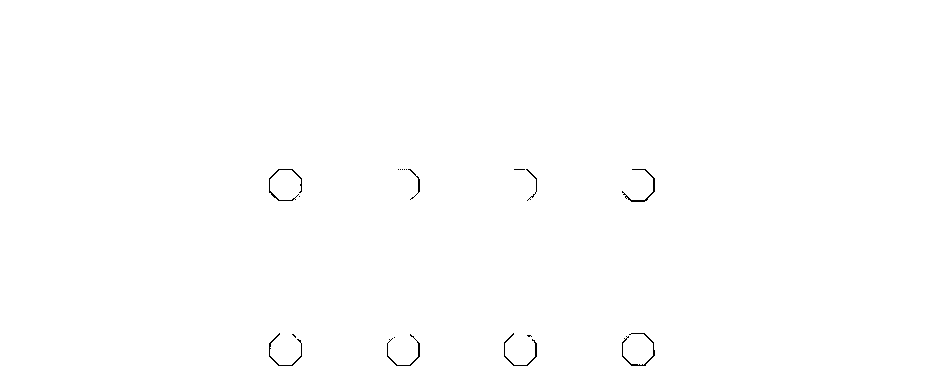
\includegraphics[width=0.2\textwidth]{image_slice_0951.png}} \\
(c) & (d)
\end{tabular}
\end{center}
\caption{The set of slices corresponding to the four projection planes in
\Figa{slice_slab}.}
\label{fig:slicing}
\end{figure}

Without loss of generality, the $y-$axis is used to represent the bottom-up direction.
Over each slab in height range $[H_{lo}, H_{hi})$,
we project the 3D data $\boldsymbol{P}(x,y,z)$, for $H_{lo} \leq y < H_{hi}$,
onto a 2D image slice.
The projection is normalized in the range $[0,W]$, where $W$ is the image width:
\begin{equation}
[\,x^{2D},\; y^{2D}\,]^T = \omega\cdot[\,x^{3D}_i - X_{MIN},\; z^{3D}_i - Z_{MIN}\,]^T
\label{eq:image_slicing}
\end{equation}
Note that $\omega = W/(X_{MAX} - X_{MIN})$, and that
the [$X_{MIN}$, $X_{MAX}$] and [$Z_{MIN}$, $Z_{MAX}$] pairs define the
3D bounding box, which can be obtained through user input and can be used
to clip away noise data.
\Fig{slicing}(a)-(d) show some examples of the 2D slices, where noise
and incomplete data are observed.
We repeatedly sweep through the volume to extract parallel volumetric slabs
along the directions of the major plane normals computed in \Sec{major_plane}.
\Fig{HT_BPA_Curvature}, for example, depicts slices extracted from the side view.

\subsection{Filling Missing Data}
\label{sec:mdr}

Extracted slices often have missing data due to occlusion or other
visibility issues.
Fortunately, most urban buildings have symmetry that we can exploit to
fill these gaps.
Symmetry computation on 3D data is expensive \cite{Sym_PSGRF},
so we conduct this computation on the 2D image slices.
Since the 3D data has been already rectified during the registration process
and projected onto 2D slices \cite{Stamos08},
symmetry computation now only needs 2D translation.
Let $P(x,y)$ be a point on the original image $I$ and $P'(x',y')$ be the reflected
point of $P$ with respect to a symmetry line $L$.
The symmetry computation equation for $L$ is as follows:
\begin{equation}
L = \underset{x,y}{\operatorname{arg\,min}}\sum{d_{x,y}(P', I)}
\end{equation}
where $d_{x,y}(P',I)$ is the distance between the self-reflected point
$P'$ and its nearest data point in image $I$.
The reflected point $P'$ of the original point $P$ is computed with
respect to a line along either the $x-$ or $y-$ axis.
Therefore, the symmetry line $L$ is obtained as the line with minimum
summation error over the reflected data points.
\Figa{sym} and \Figb{sym} depict the original input with missing data, and
the output after gap filling using symmetry computation, respectively.

\begin{figure}[htbp]
\begin{center}
\begin{tabular}{cc}
\fbox{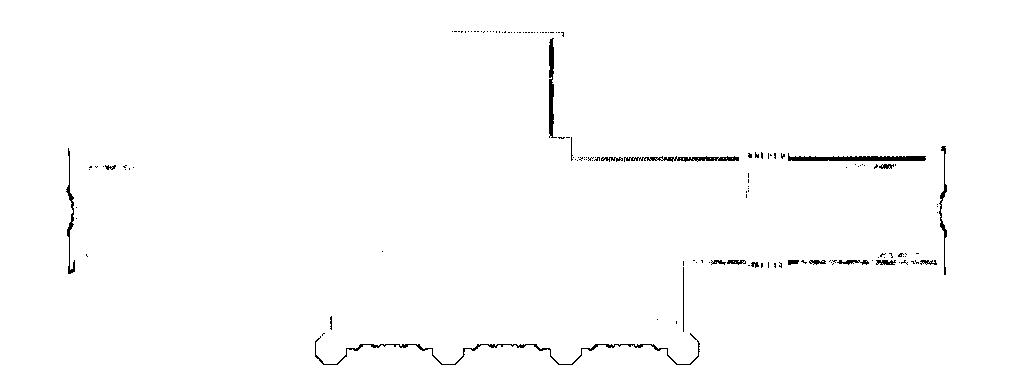
\includegraphics[width=0.2\textwidth]{image_slice_0705_0711.png}} &
\fbox{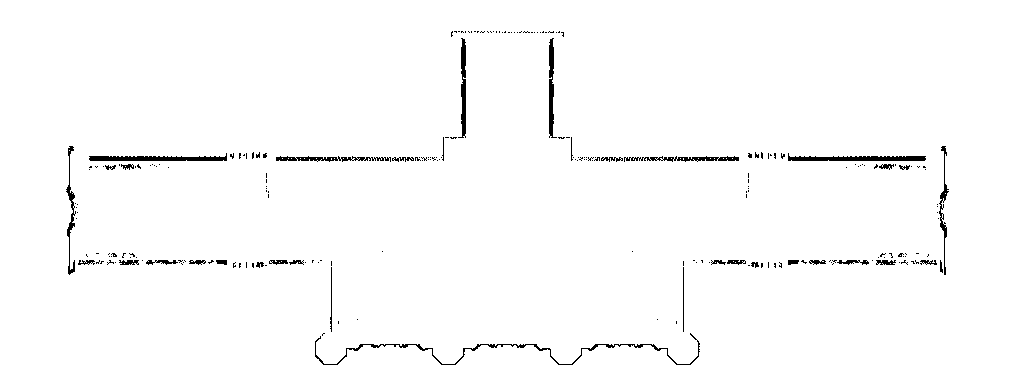
\includegraphics[width=0.2\textwidth]{image_slice_0705_0711_recoverd.png}} \\
(a) & (b)
\end{tabular}
\end{center}
\caption{ Symmetry-based gap filling. (a) Original 2D slice image and
(b) output image after gap filling.}
\label{fig:sym}
\end{figure}

\subsection{Dataset Segmentation}
\label{sec:mseg}

Modeling the PCD of a building as a whole structure simultaneously
is complicated due to the natural complexity of buildings.
To simplify this problem, we utilize the divide and conquer strategy
to segment the whole PCD into simpler parts.
Each of these parts can be easily represented by extrusion/taper operations.
3D PCD segmentation is generally performed using region based methods,
although their computational cost may be high.
We propose an efficient segmentation approach based on the observation
that different parts of a building are usually separated by walls, ledges,
and other architectural elements.
These {\it ``separators''} provide segmentation clues.

To detect these separators, we examine the data point distribution of 2D
slices extracted from all major planes, as depicted in \Fig{plot_seg}.
We identify the separators as the indices of the slices that coincide
with the local maxima and inflection points in the data point distribution.
Once we obtain the separators, we can segment the original dataset based on
the intersections of these separator planes.
As \Figb{slice_slab} shows, there are a total of five regions that are
identified for the PCD shown in \Figb{IR_2_DXF}, where each segment is
labeled with a different color.

\begin{figure}[htbp]
\begin{center}
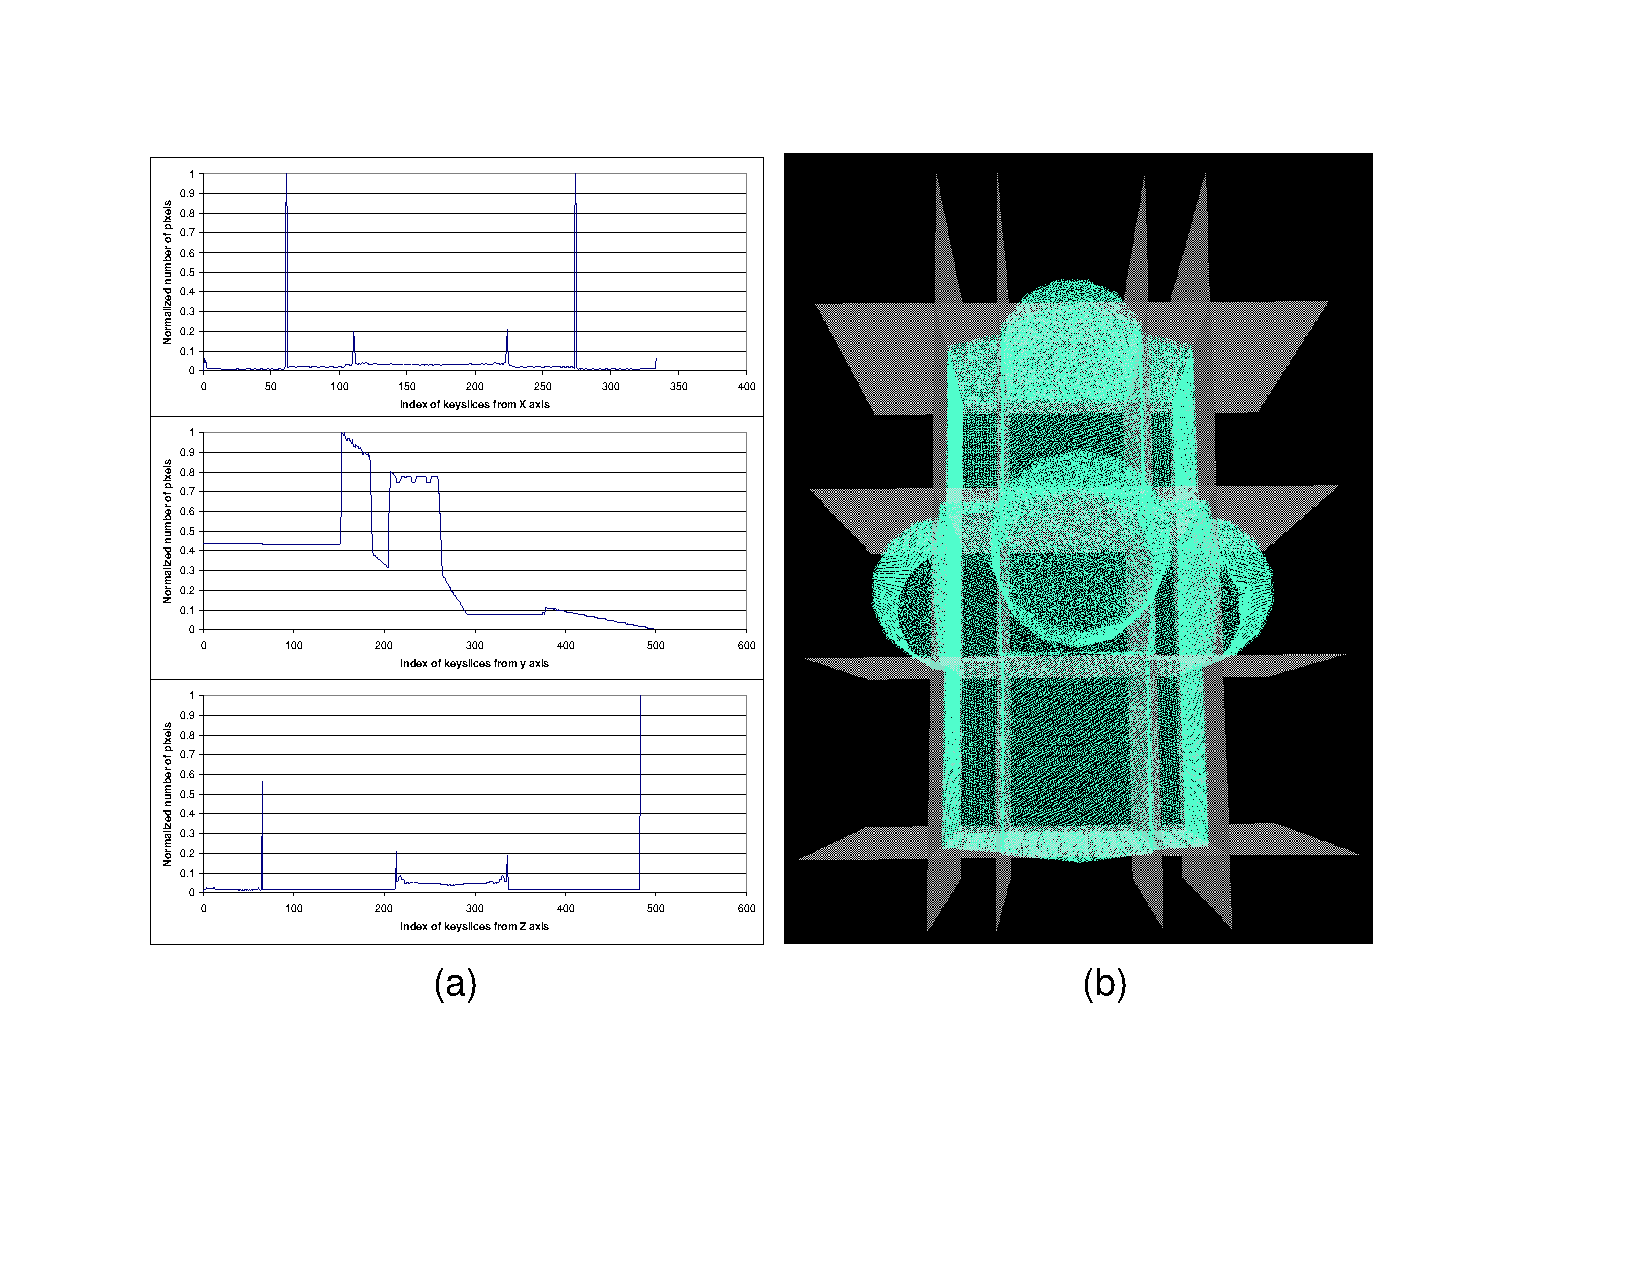
\includegraphics[width=0.48\textwidth]{plot2.pdf}
\end{center}
\caption{
The distribution of data points in cross-sectional slices along X, Y, and Z axes
for the model shown in the second row of \Figb{results}.
The distribution is defined as the sum of pixels of each cross-sectional slice.
(b) Top view of the point cloud with cutting planes inserted at the extremas
of the point distributions shown in (a).
}
\label{fig:plot_seg}
\end{figure}

% When projected onto 2D images, these separators have a common characteristic,
% that is a relative large {\it ``dark''} region
% representing a salient feature in binary images.
%
% We used a kernel based connected components (CC) method for separator detection.
% For each projected slice image $I_i$, the separator detector
% checks each data point $P_i$ using a $5$x$5$ kernel $K$ centered at $P_i$.
% When there is no more new data point covered by $K$,
% the detector stops with a new connected component, $C$, being found.
% As a verification step, the size of $C$ is checked to ensure
% that it contains a big chunk of data, that is, a {\it dark} region.
% Occasionally, separators might be detected in adjacent or neighboring sliced images,
% which usually caused by imperfect PCD registration introduced in earlier stages.
% For this case, we integrate all those neighboring sliced images
% as a new sliced image $I$.
% And the same separator detection algorithm is applied on $I$
% to obtain the bounding information.
%
% To conduct the segmentation, we need to transform the separators in all directions
% into the common coordinate (with $y$-axis as the bottom-up direction).
% Each separator will be transformed into a line segment in the bottom-up
% projected image with the end points representing the bounding positions.
% The goal is to compute the regions generated by the intersections of those line segments.
% To do this, we can compute intersection points for each line segment
% with other line segments and then compute the regions bounded by these intersection points.
% Once we obtain the segmentation regions, it is trivial to segment the PCD into those regions.
%

%%%%%%%%%%%%%%%%%%%%%%%%%%%%%%%%
%%%%%%   3D Reconstruction  %%%%
%%%%%%%%%%%%%%%%%%%%%%%%%%%%%%%%
\section{Lightweight 3D Reconstruction}
\label{sec:reconst}
Our 3D modeling algorithm is based on \emph{a priori} knowledge that
urban buildings can be created through a series of extrusion and tapering
operations on the salient cross-sections contained in the keyslices.
The main step for successful modeling is identifying these salient cross
sections upon which the extrusion and tapering operations apply.

\subsection{Window Detection}
\label{sec:win_detect}
Windows and doors are important features for buildings to be modeled.
Moreover, accurate computation of the extrusion structures depends on this information.
Without knowing the locations of the windows, extra keyslices may be computed
hence leading to excessive extrusion operations on windows.
Our window detection algorithm is based on the work presented in \cite{WDD_PV}.
Following this, we can generate mask images based on the boundaries of the
detected windows to discard the 3D points in the window regions for keyslice
computation.

During the window and door detection step, we retain the boundary, position,
and depth of the windows. 
After the facade is extruded from one keyslice to the next (see \Sec{ksd}),
we project the boundary of the window/door onto the extruded facade.
This projected boundary is pushed into the facade in the opposite direction
of the face normal up to the recovered depth of the window.
This action significantly reduces the number of polygons from the model.

\subsection{Keyslice Detection}
\label{sec:ksd}

The 2D image slices of an extruded region are similar to each other.
Thus, to detect the keyslices that delimit extruded regions one only needs
to compute the similarity between adjacent slices.
We adopted a light-weighted global and efficient key image detection approach
based on distance function similar to
Hausdorff distance as the similarity measure.
Let $P_r(x_r, y_r)$ and $P_i(x_i, y_i)$ be a data point in
a reference image and a new observed image $I$, respectively.
The distance function of image $I$ to reference image $I_r$ is defined as:
\begin{equation}
d_H(I, I_r) = \sum_{i=0}^Nd_{min}(P_i, I_r)
\label{eq:hd}
\end{equation}
where $d_{min}(P_i, I_r)$ is the minimum distance from $P_i$ in image $I$
to the reference image $I_r$.
Alternatively, we can also define the distance, $d_H(I_r, I)$,
from $I_r$ to a new observed image $I$, using \Eq{hd}.
These two distances are usually not equal to each other.
As a rule of thumb, one can choose
$d_{HD} = \text{MAX}\{d_H(I, I_r), d_H(I_r, I)\}$ as the distance.
To compute the keyslices, a threshold $\tau_{d}$ is used for the
distance $d_{HD}$.
If $d_{HD} < \tau_{d}$, the two images $I$ and $I_r$ are considered
similar to each other.
Otherwise, a keyslice image is found and $I_r$ is updated with $I$,
the new keyslice image.

The accuracy of the keyslices detected by using the distance function
is closely tied to threshold $\tau_d$.
Small $\tau_d$ leads to more accurate models and will require more time and
space to compute and store the result.
When the threshold $\tau_d$ is relatively large, potential keyslices which
contain salient structure may be missed.
Therefore, there is a trade-off between model accuracy and time-space
efficiency.
To address this problem, the curvature information is computed as a
complementary criteria for keyslice detection.

This idea is based on the observation that the keyslices are generally
located at large curvature changes along 2D slices extracted in the orthogonal
direction (e.g., side view), as shown in \Fig{HT_BPA_Curvature}.
Therefore, instead of computing the difference between two images directly,
we compute the curvature of orthogonal 2D slices, map the positions of
curvature extrema back to cross-sections in the original set of volumetric
slabs, and mark these cross-sections as keyslices.

\begin{figure}[htbp]
%\begin{center}
\centerline{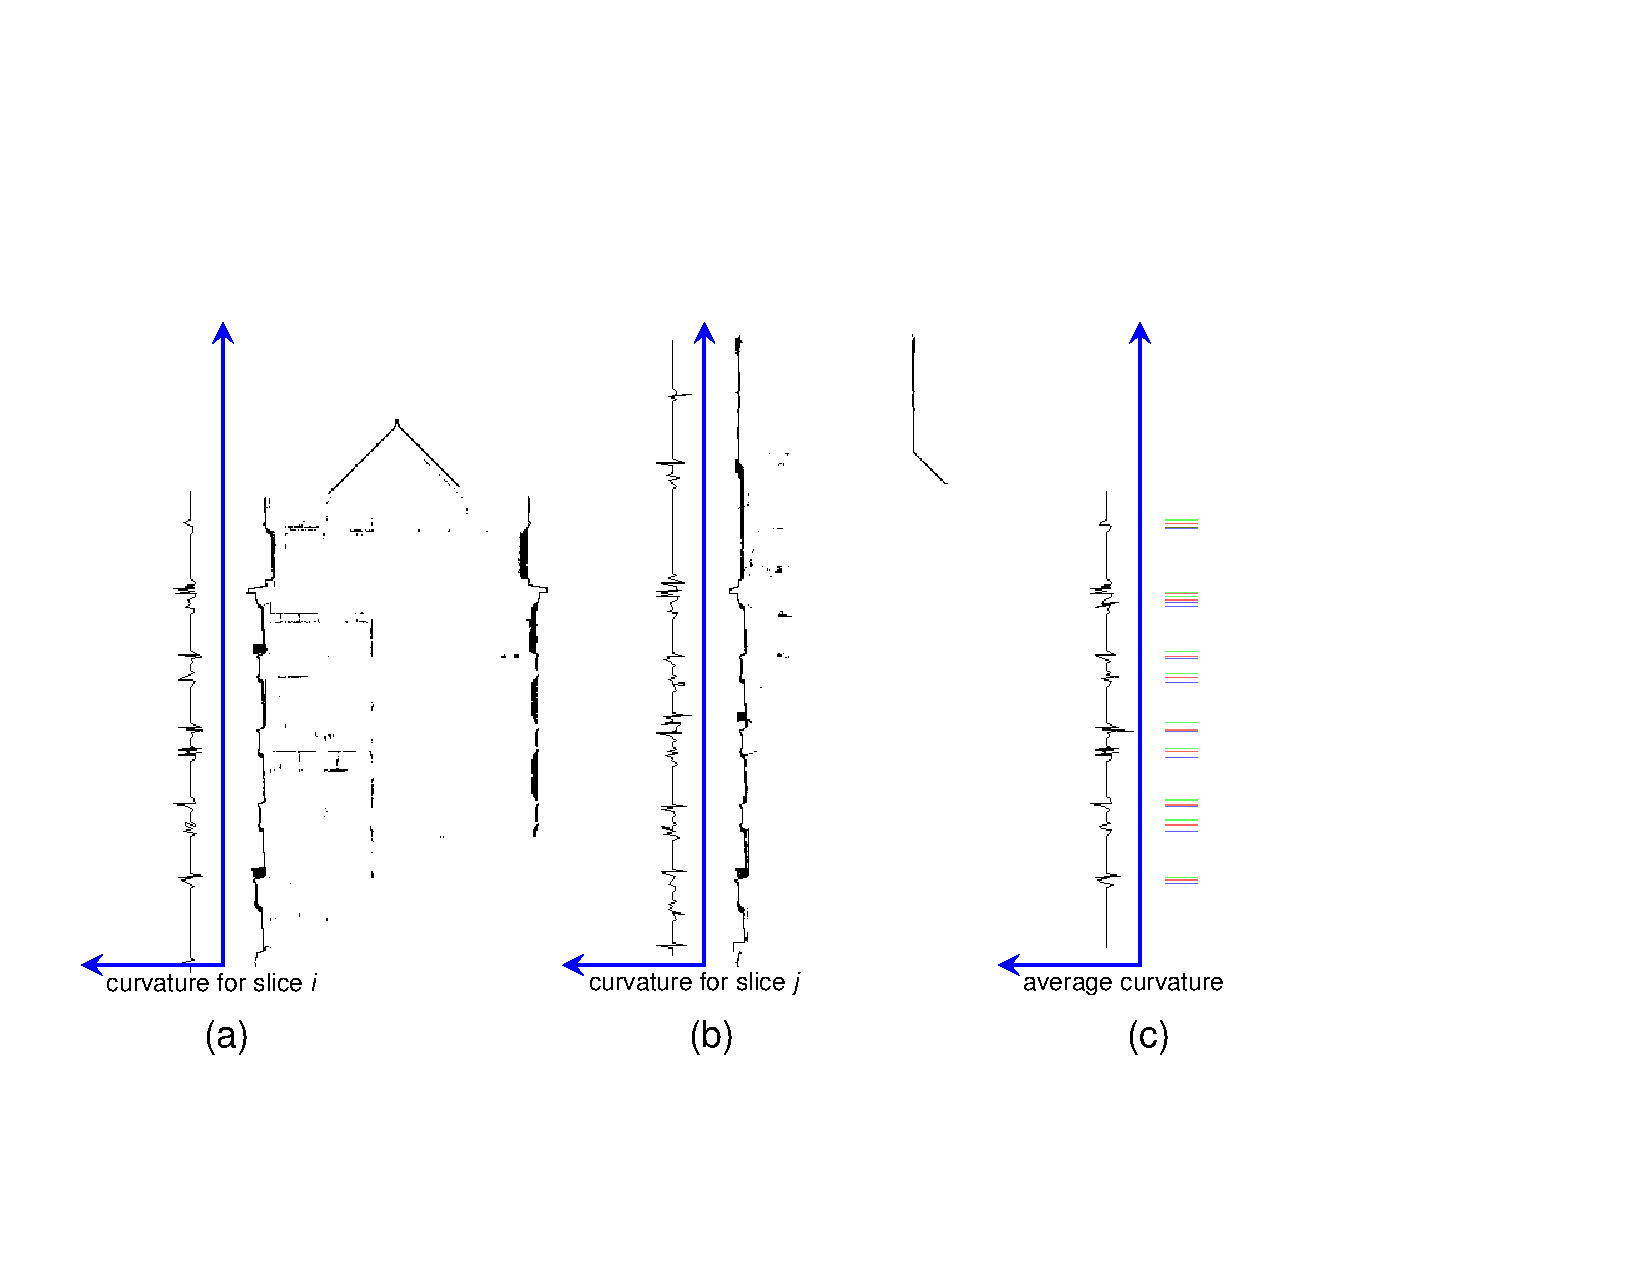
\includegraphics[width=.5\textwidth]{curvature_comp.pdf}}
%\begin{tabular}{cc}
%\fbox{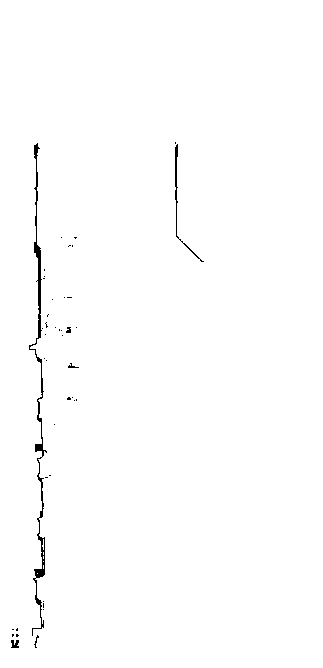
\includegraphics[width=0.12\textwidth]{image_slice_lr_0580_0590_half.png}}
%\fbox{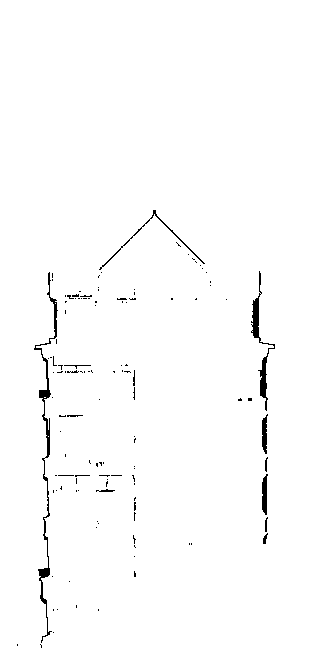
\includegraphics[width=0.12\textwidth]{image_slice_lr_0830_0842_half.png}} &
%\fbox{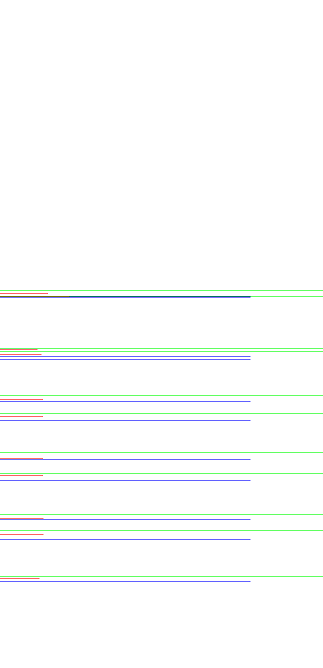
\includegraphics[width=0.12\textwidth]{curvature_center_lines_old_half.png}} \\
%(a) & (b)
%\end{tabular}
%\end{center}
\caption{Curvature-based key slice detection.
(a,b) Two 2D sliced images from the orthogonal direction (side view).
A plot of the curvature of each slice is displayed alongside.
(c) A plot of the average curvatures detected over all of the sliced
images along the orthogonal direction.
Thresholding the curvature yields the location of keyslices, displayed
alongside the plot.
Red lines along the average curvature plot indicate local maxima.
Blue and green lines, respectively, indicate zero-crossings in the
average curvature.
This delineates the keyslice positions.
}
\label{fig:HT_BPA_Curvature}
\end{figure}

To compute the curvature, we first apply the slice extraction algorithm
described in \Sec{image_slicing} to obtain a series of 2D cross-sectional
images in the orthogonal direction.
We then apply the ball-pivoting algorithm described in \Sec{BPA} to
vectorize the boundary for each sliced image.
We locate those curvatures that appear in most of the sliced images as the
places where keyslices are found, as shown in \Figc{HT_BPA_Curvature}.
The combination of similarity measure and curvature inference
ensures that the salient structures of a building will be preserved.

\subsection{Boundary Vectorization}
\label{sec:BPA}

After the keyslices are detected, $K$ keyslices will be identified
from a total of $A$ image slices.
Depending on the threshold $\tau_{d}$, $K$ is usually about one to two
orders of magnitude smaller than $A$, e.g., $K/A$ is 0.06 when
$\tau_d$ = 4.0 for the example in \Figb{IR_2_DXF}.
To generate the 3D model, these keyslice images need to be vectorized to
represent the contours of the building facade.
The Douglas-Peucker algorithm attempts to connect all of the existing points
to form a polygon \cite{DP_DP}.
Although the implementation of this approach is very efficient with the
improvement described in \cite{DP_HS}, this method cannot handle the case
where spurious interior points are present, which contributes to outlier data.
To tackle this issue, we adapted the ball-pivoting algorithm (BPA)
\cite{BPA_BMRS} from its original use on 3D PCD to use on
2D keyslice images where it produces vectorized boundaries.
The key parameter for the BPA algorithm to work successfully is to
find the right size of the ball for pivoting.
We implemented a coarse-to-fine adaptive BPA algorithm to solve this problem.

\subsection{Extrusion and Taper Detection}
\label{sec:tsd}

After the keyslices are detected and vectorized, the contours of
the set of $K$ keyslices are used to represent the building based
on the extrusion operation.
That is, the space between each adjacent pair of keyslices
is filled by extruding one keyslice to the next.
By modeling a building using extrusion operations on the keyslices,
we significantly reduce the number of polygons for urban buildings.

In addition to the extrusion operation, we can further improve
the model and reduce the model size based on the observation
that part of the keyslice images may belong to the same tapering structure.
The difficulty in inferring tapering structures is tied to
the complexity of a building structure itself.
Fortunately, the dataset segmentation module introduced in \Sec{mseg}
has segmented the complicated structures into simpler parts.
Although the majority of building tapering structures are {\it linear tapering},
such as {\it tapering to point} (TTP), a cone shape geometry,
and {\it tapering to line} (TTL), a wedge shape,
it could also be a complicated {\it non-linear tapering},
such as a dome shape.
Furthermore, a structure may look like a tapering structure,
but it is actually not a real one.
For example, a series of small extruded structures
form a tapering-like shape.

We introduced a two-step workflow to accomplish the above goal.
The first step is to locate the potential tapering keyslices
and infer the structure by making an assumption that
the underlying tapering structure is either a TTP or a TTL.
A verification step is conducted to check the correctness
of the inferred shape by measuring the error between the model and
the corresponding 3D PCD.
If the error is small, the inferred shape is confirmed
and the underlying keyslices are not rendered.
Otherwise, we can choose to model this special structure by fitting a
triangular mesh to the underlying 3D point cloud to produce a polygonal model.
This algorithm cannot model a sphere or a dome because such structure
cannot be linearly interpolated as a taper operation.

% The assumption of linear tapering to a line or point makes the
% tapering structure inference much simpler and more efficient.
% For a keyslice set ${\bf N_K} = \{I_i | 0 \le i \le N \}$,
% where $i$ is the projected slice index, we first compute
% the sets of keyslices for potential tapering structures.
% This is based on the observation that for tapering structures,
% the underlying keyslices indices form nearly an arithmetic progression.
% The keyslice set ${\bf N_T}$ indicates a potential section of a
% tapering structure in the projected range.
% ${\bf N_T}$ also provides a very important information for inferring the
% underlying structure: based on the assumption, the first element, $I_0$,
% in ${\bf N_T}$ is the base geometry shape for the linear tapering structure.
% And the last element, $I_f$, of ${\bf N_T}$
% is the converged or partially converged geometry shape.
% If $I_f$ contains either a line segment or a point structure,
% this indicates that the underlying tapering structure of ${\bf N_T}$
% is completely converged.
%
% The basic idea for the verification stage is to measure the error
% for the new inferred tapering structure.
% The error is defined as the distance $d_e$ between a 3D point $p$ and
% the inferred model $M$.
% If $d_e$ is smaller than a threshold, $t$, the tapering structure is approved and
% the corresponding keyslices are substituted to further compress the model.
% Otherwise, the underlying tapering structure is rejected.
% We chose $t = \tau_d/2$ as the threshold,
% and it worked well on our synthetic and real datasets.
% Here, $\tau_d$ is the threshold for keyslice detection
% as introduced in \Sec{ksd}.
%
%%%%%%%%%%%%%%%%%%%%%%%%%%%%%%%%
%%%%%%   Experimental Results%%%
%%%%%%%%%%%%%%%%%%%%%%%%%%%%%%%%
\section{Experimental Results}
\label{sec:IR_OUT}

To generate the final 3D model, the control
points of the 2D contours can be transformed back into 3D world coordinate system
using the reverse matrix $T$ in equation \Eq{image_slicing}.
For each segment, we first exam whether it can be modeled
by simple keyslices along any major plane.
If so, the push-pull operation is applied to the keyslice contours to
generate the extruded model.
If a tapering structure is detected, we construct the faces
based on the control points of the 2D base geometry polygon
and their corresponding converged points to create the tapering model.

\Fig{results} shows the experimental results for both synthetic (the first two rows)
and real datasets (the last three rows).
Each row shows a reconstruction of a building.
The snapshot of the original model or the image of the real building
is shown in (a), followed by the snapshot of 3D PCD in (b).
Columns (c)-(e) depict the segmentation result,
the vectorized keyslices, and the snapshot of the reconstructed model, respectively.

\begin{figure*}[htbp]
\begin{center}
\begin{tabular}{ccccc}
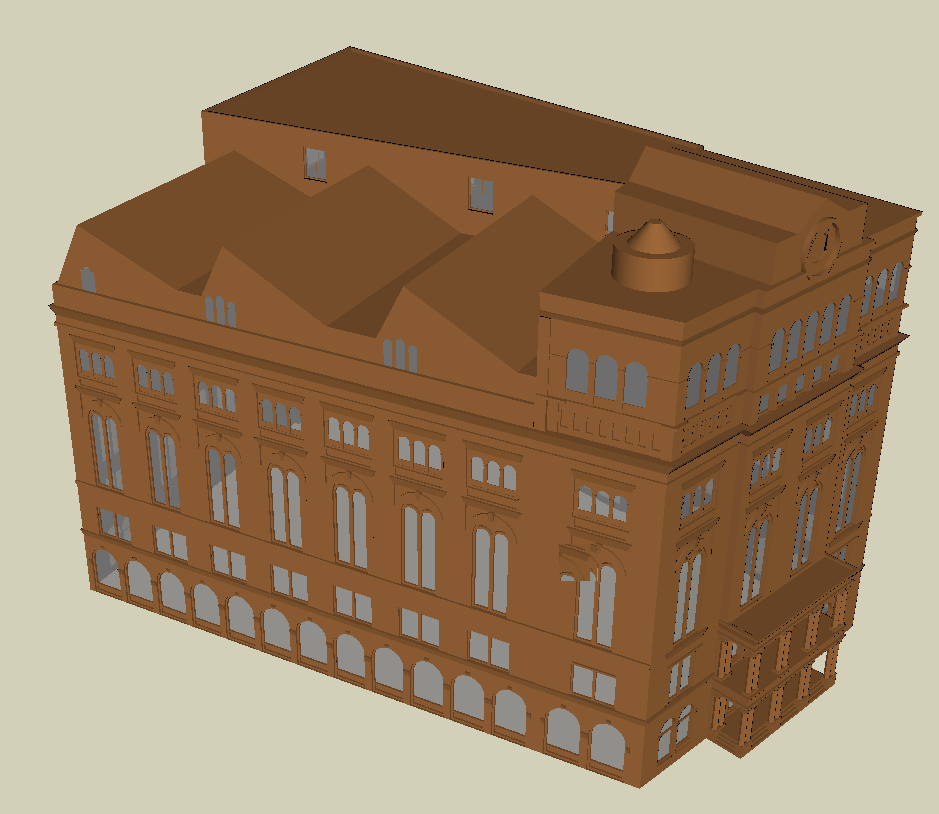
\includegraphics[width=0.18\textwidth]{cu_1.png} &
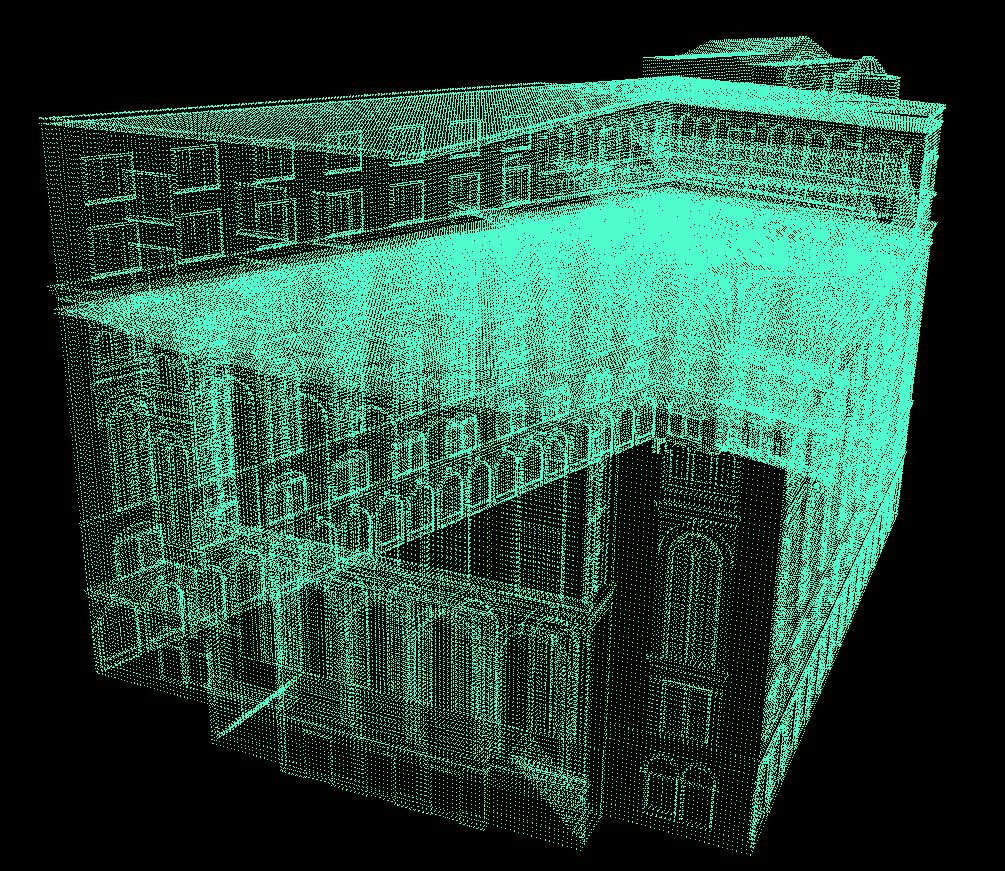
\includegraphics[width=0.18\textwidth]{cu_2.png} &
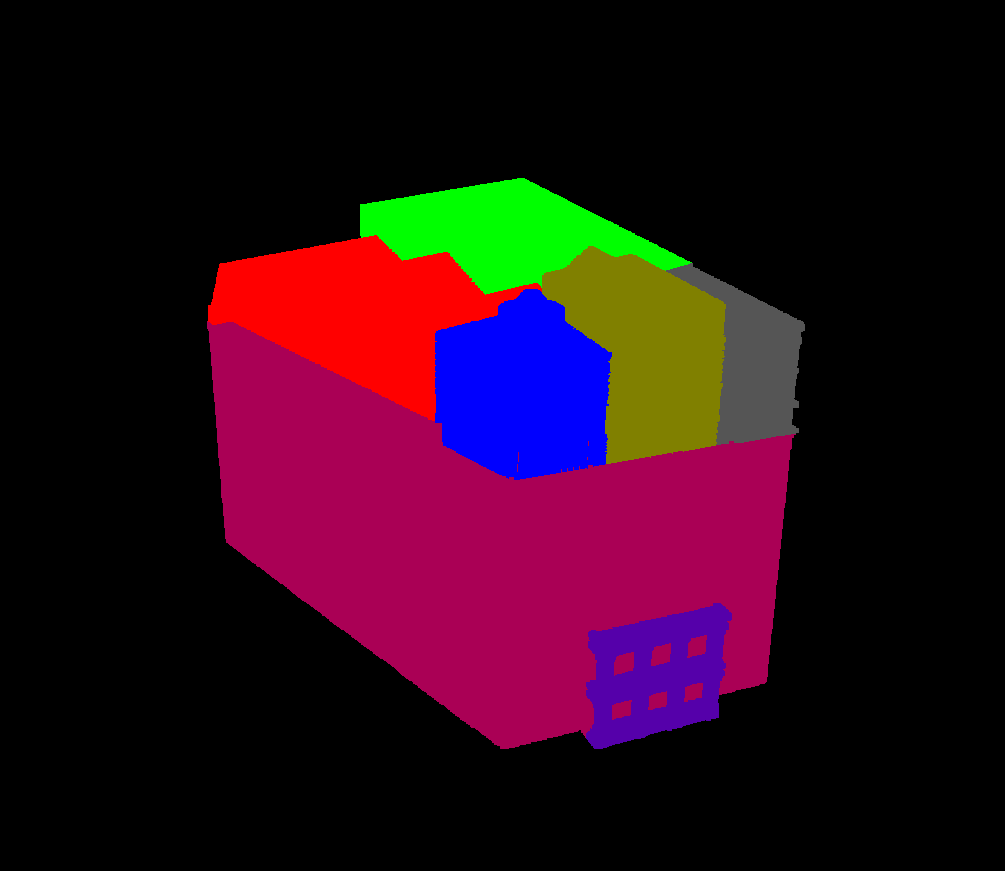
\includegraphics[width=0.18\textwidth]{cu_7.png} &
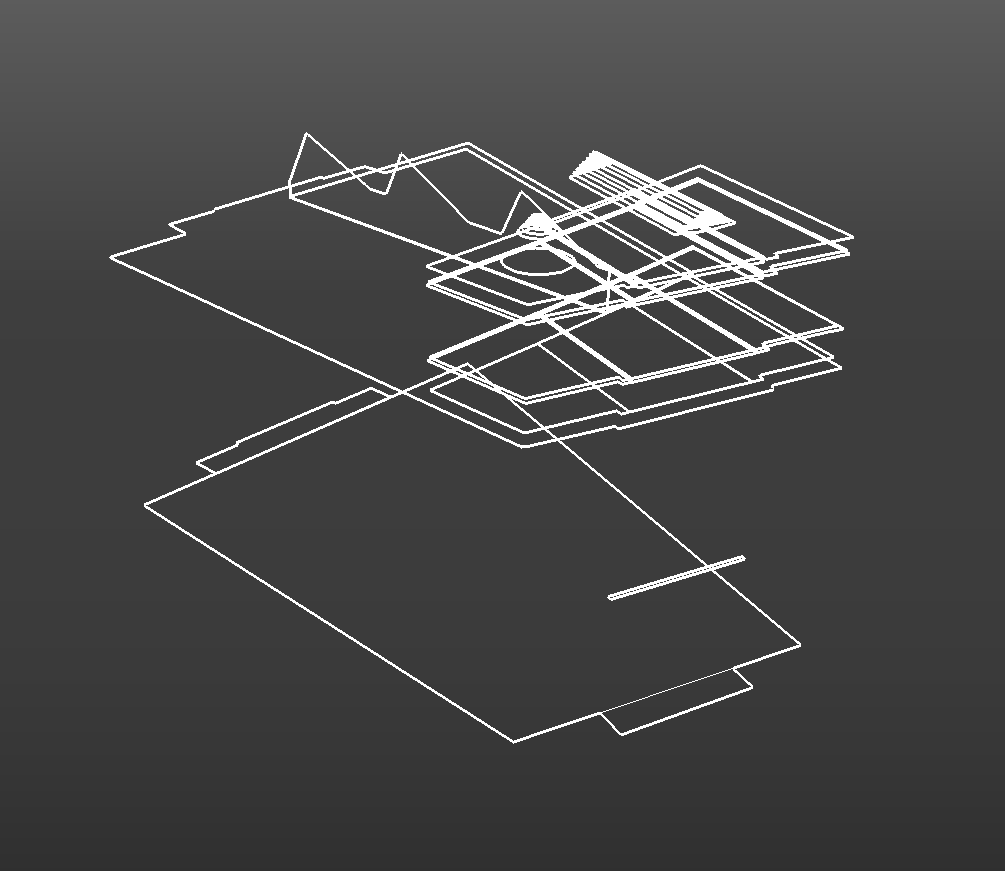
\includegraphics[width=0.18\textwidth]{cu_9.png} &
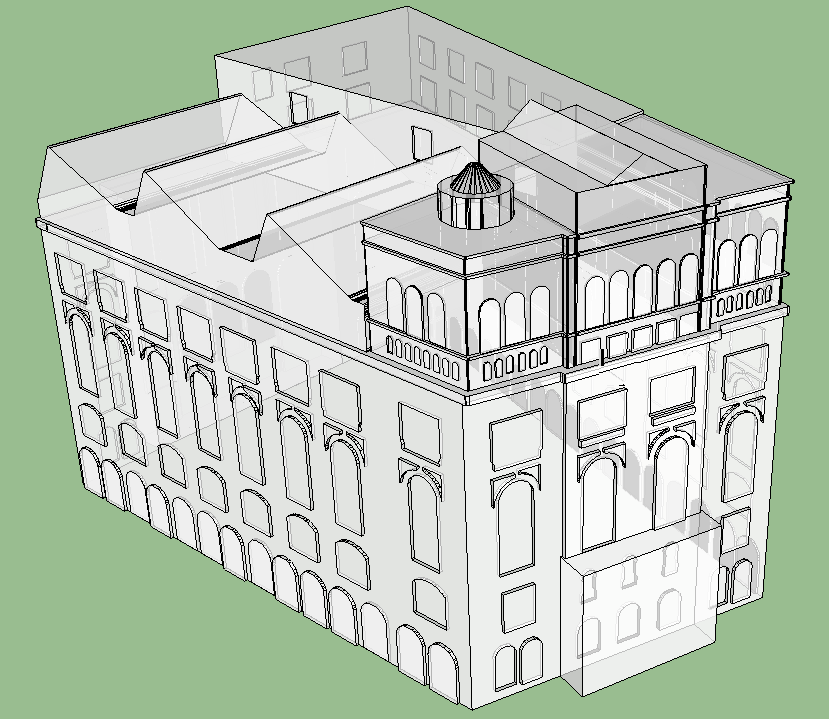
\includegraphics[width=0.18\textwidth]{cu_3.png} \\
%(a) & (b) & (c) & (d) & (e)\\
% 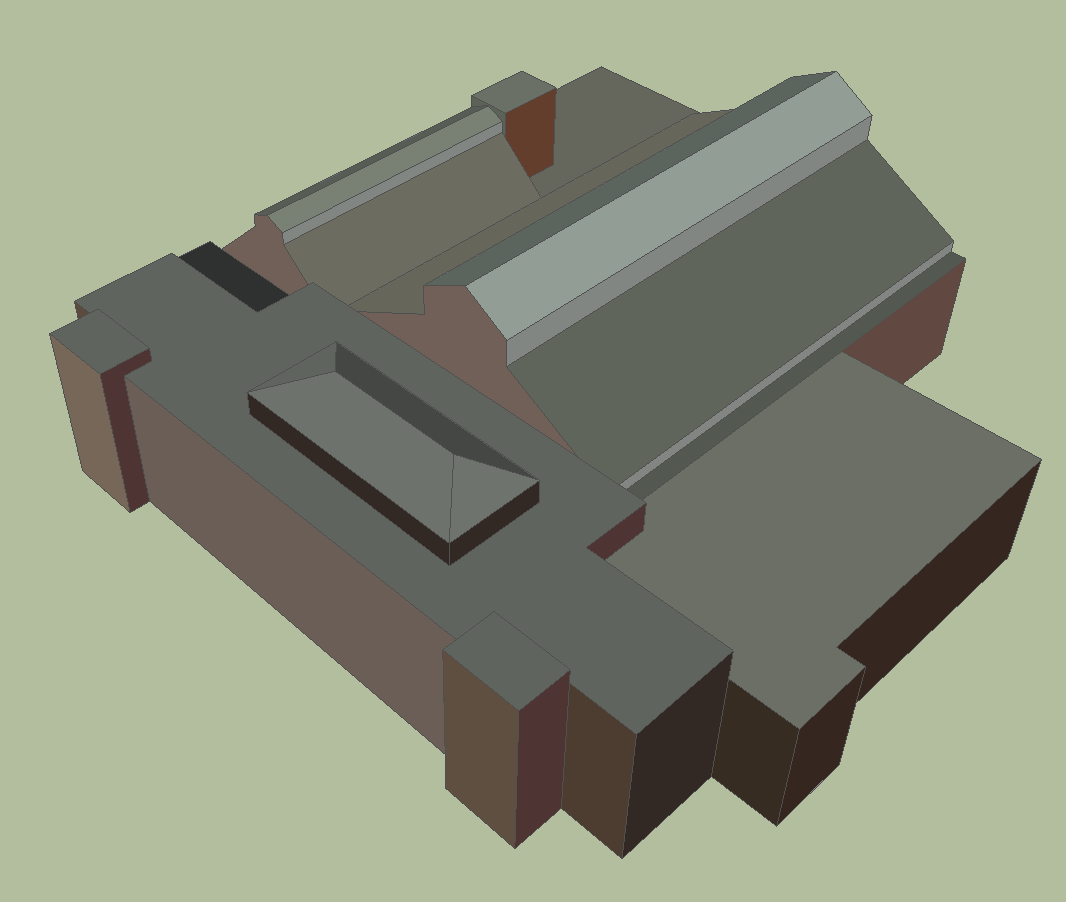
\includegraphics[width=0.18\textwidth]{health_town_1.png} &
% 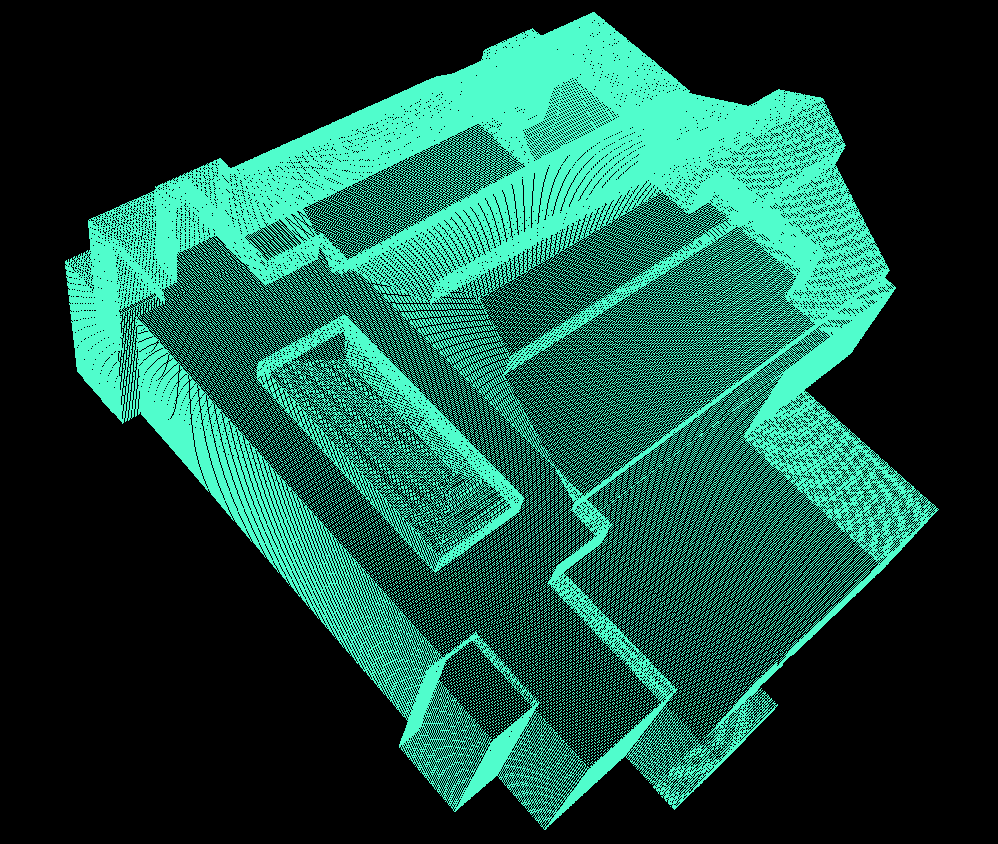
\includegraphics[width=0.18\textwidth]{health_town_2.png} &
% 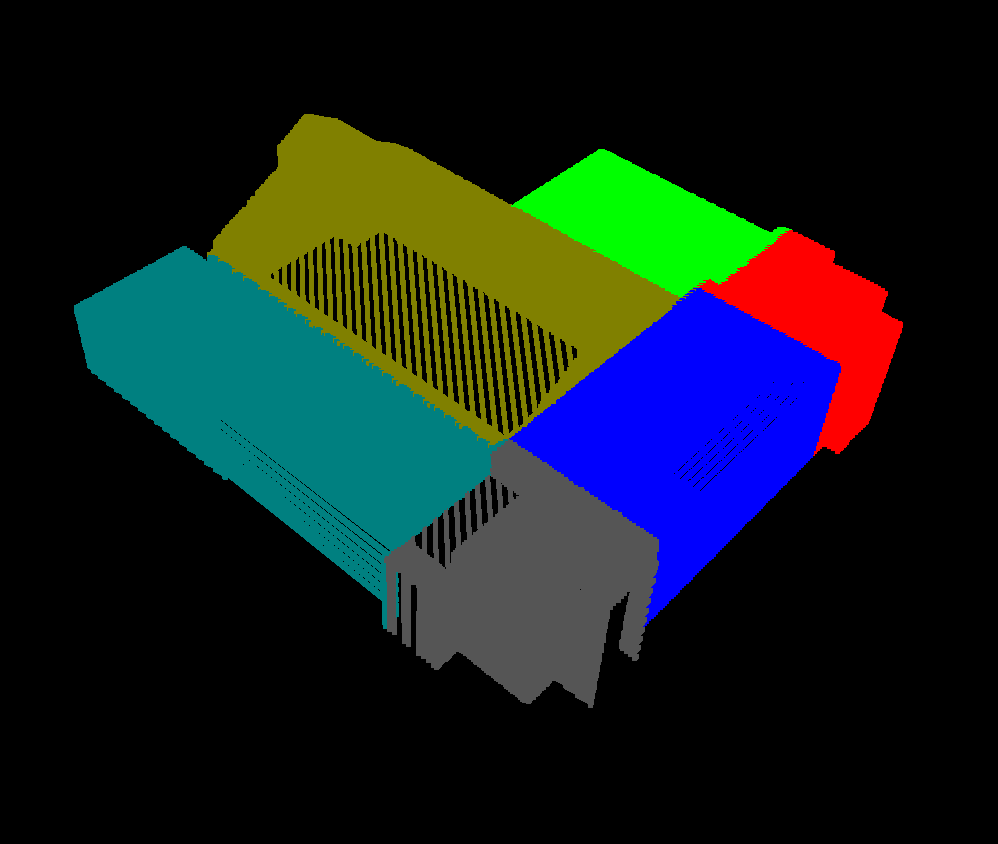
\includegraphics[width=0.18\textwidth]{health_town_7.png} &
% 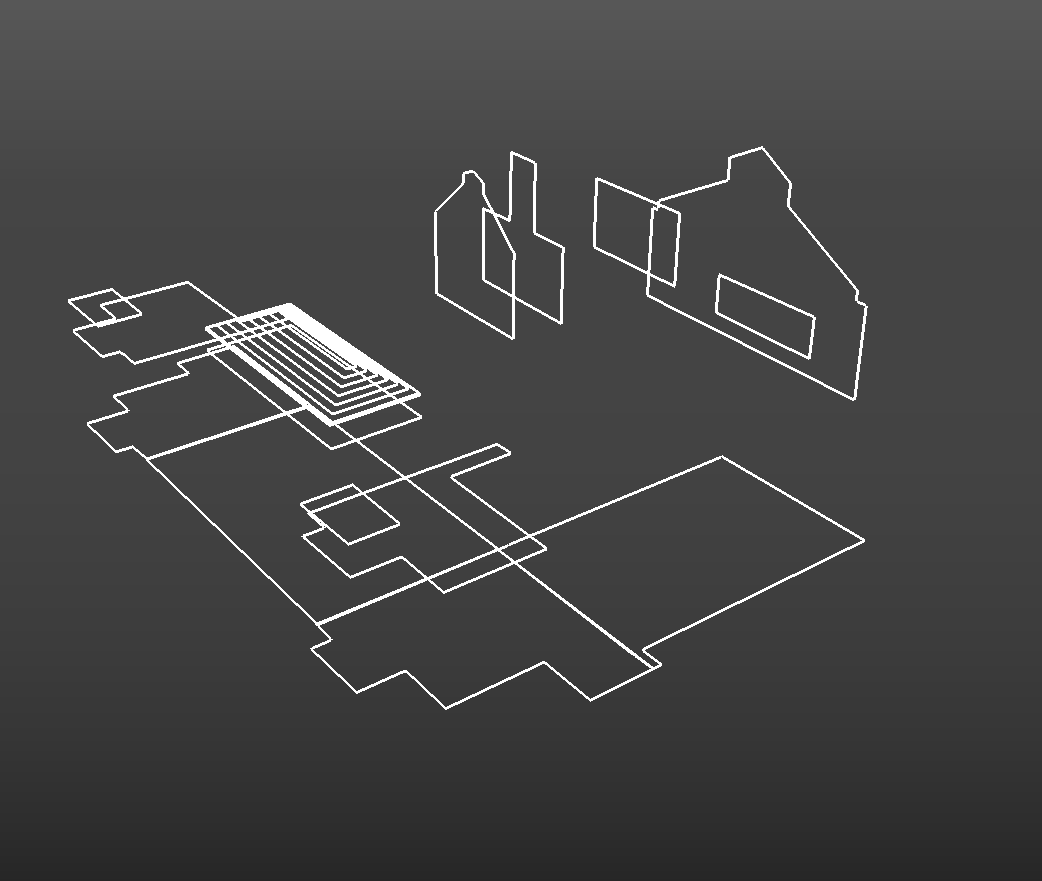
\includegraphics[width=0.18\textwidth]{health_town_9.png} &
% 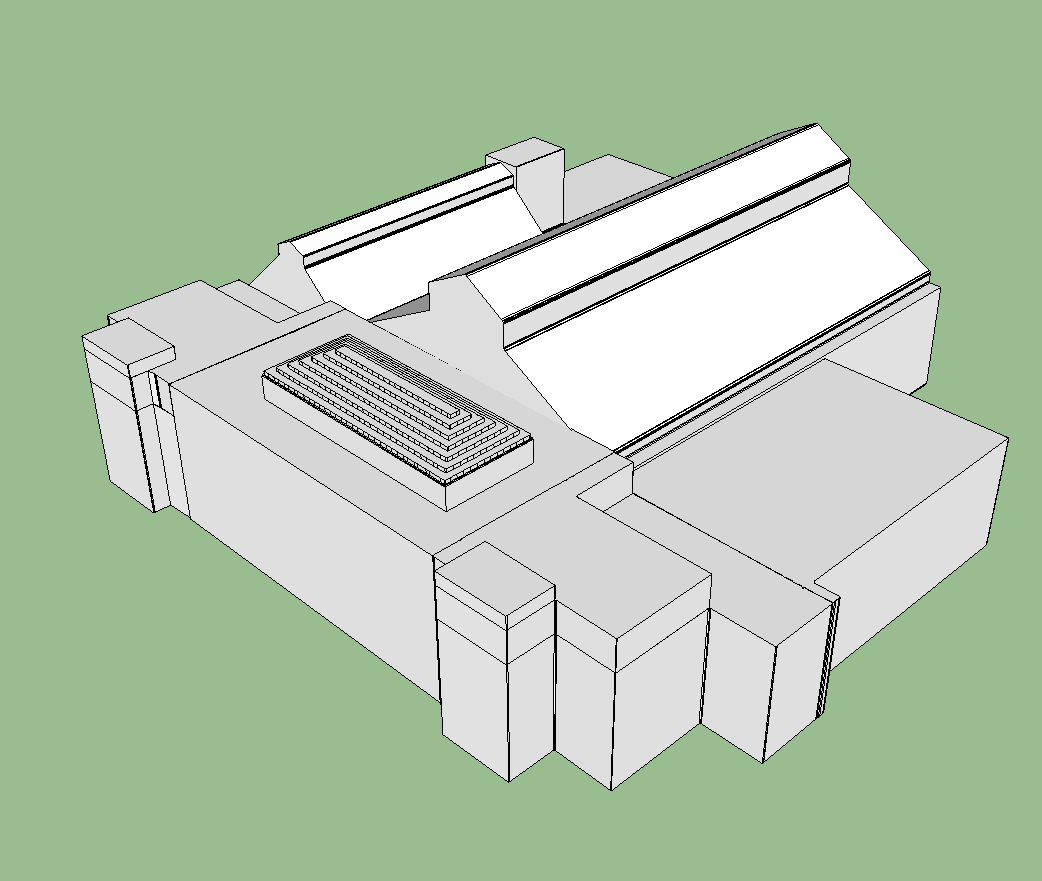
\includegraphics[width=0.18\textwidth]{health_town_11.png} &
% 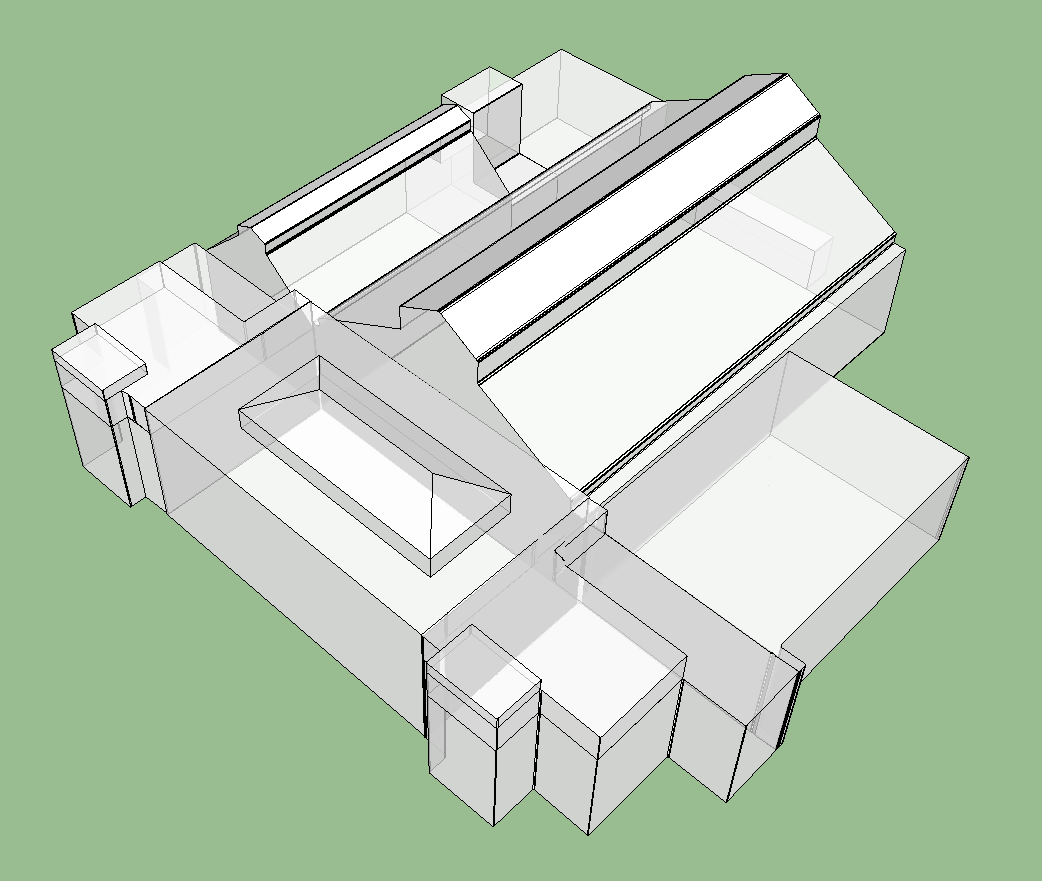
\includegraphics[width=0.18\textwidth]{health_town_3.png} \\
%(a) & (b) & (c) & (d) & (e) & (f) \\
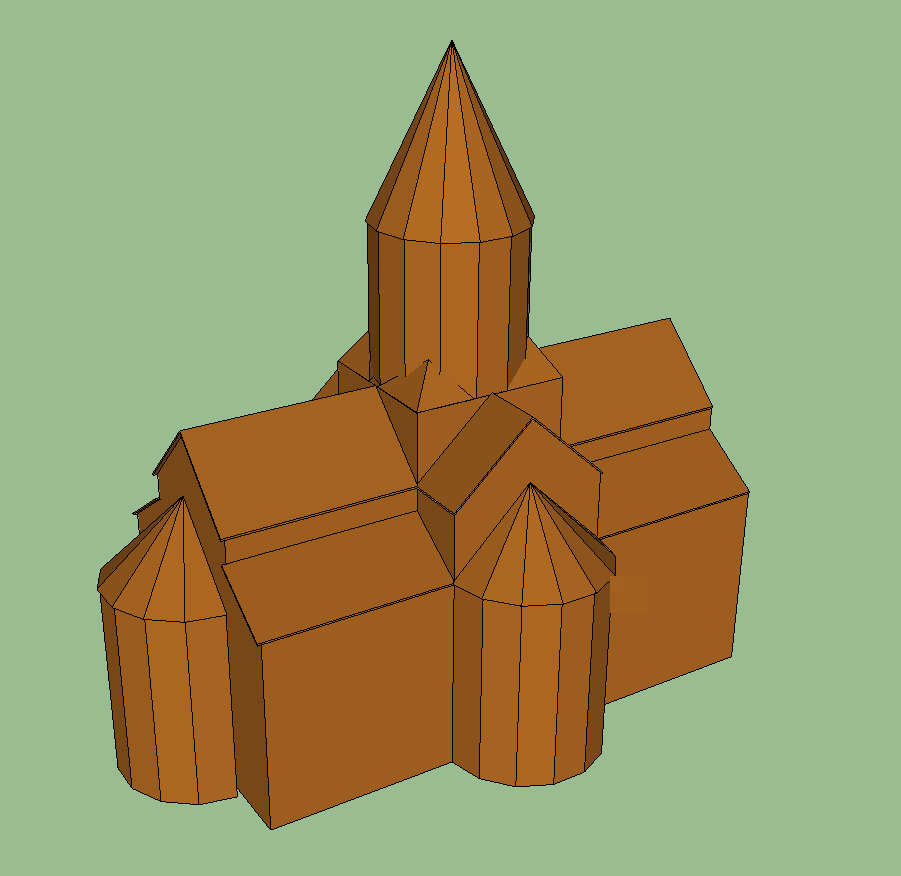
\includegraphics[width=0.18\textwidth]{spitak_1.png} &
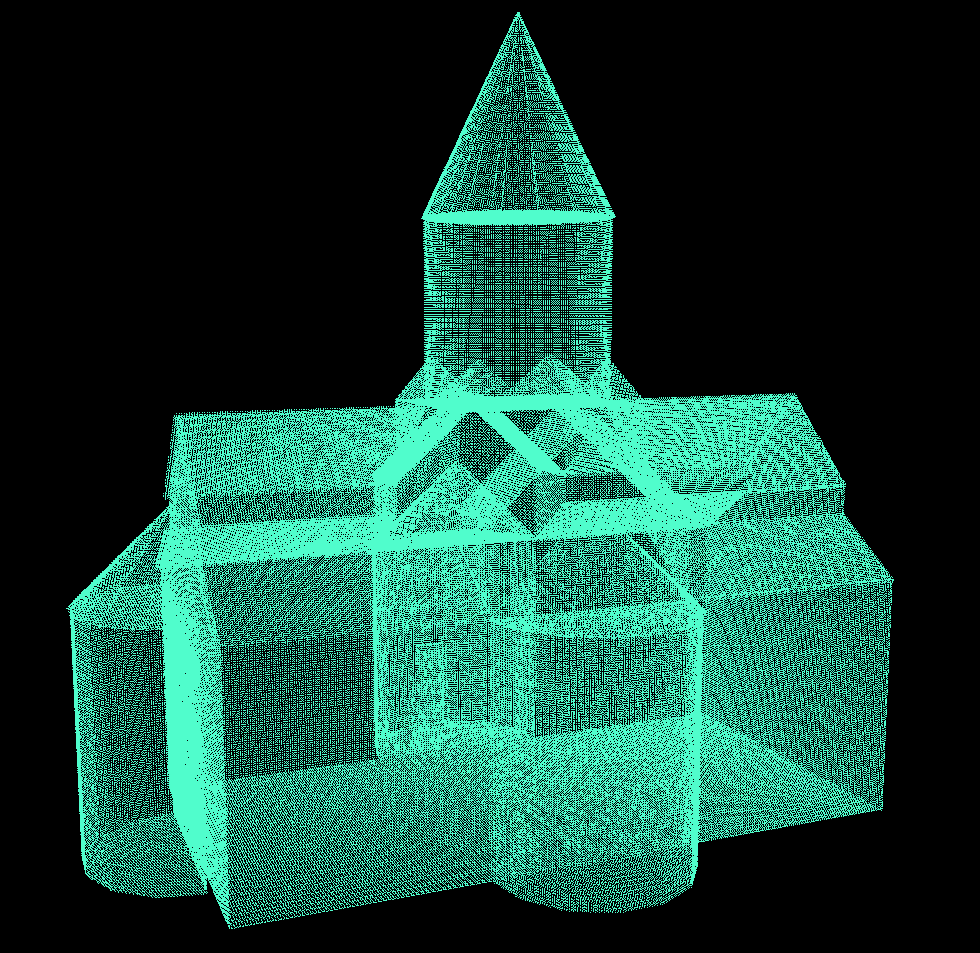
\includegraphics[width=0.18\textwidth]{spitak_2.png} &
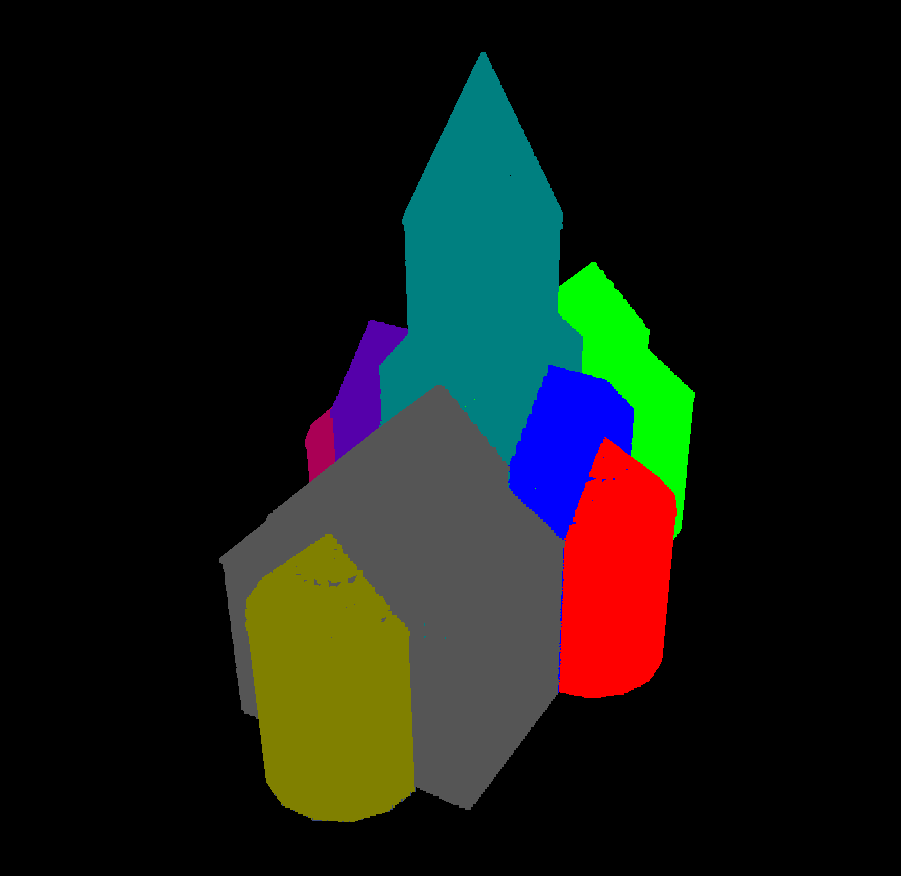
\includegraphics[width=0.18\textwidth]{spitak_7.png} &
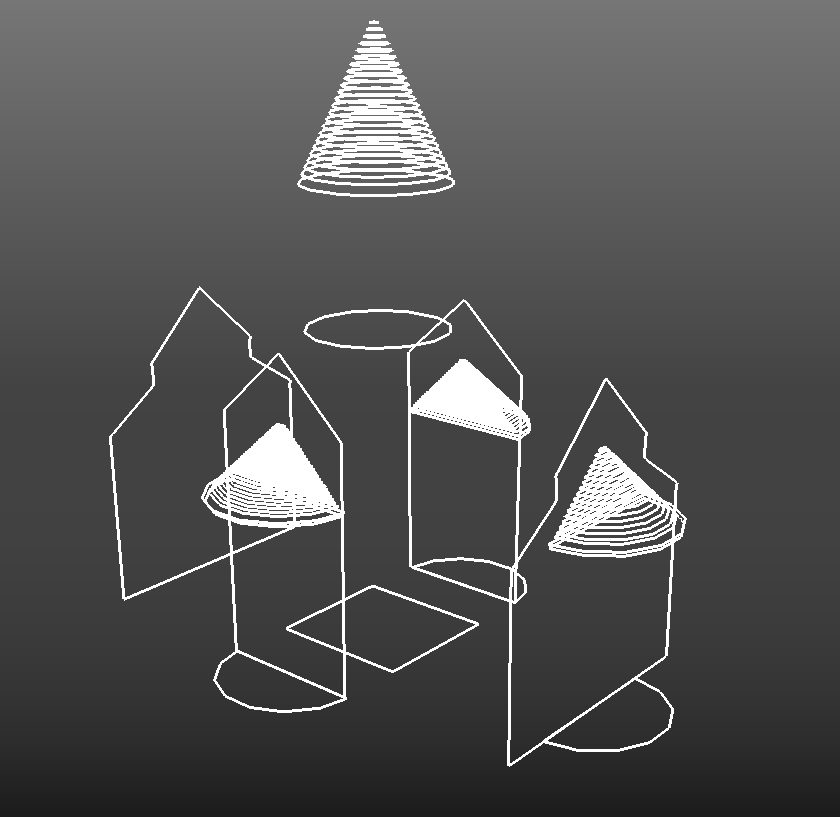
\includegraphics[width=0.18\textwidth]{spitak_9.png} &
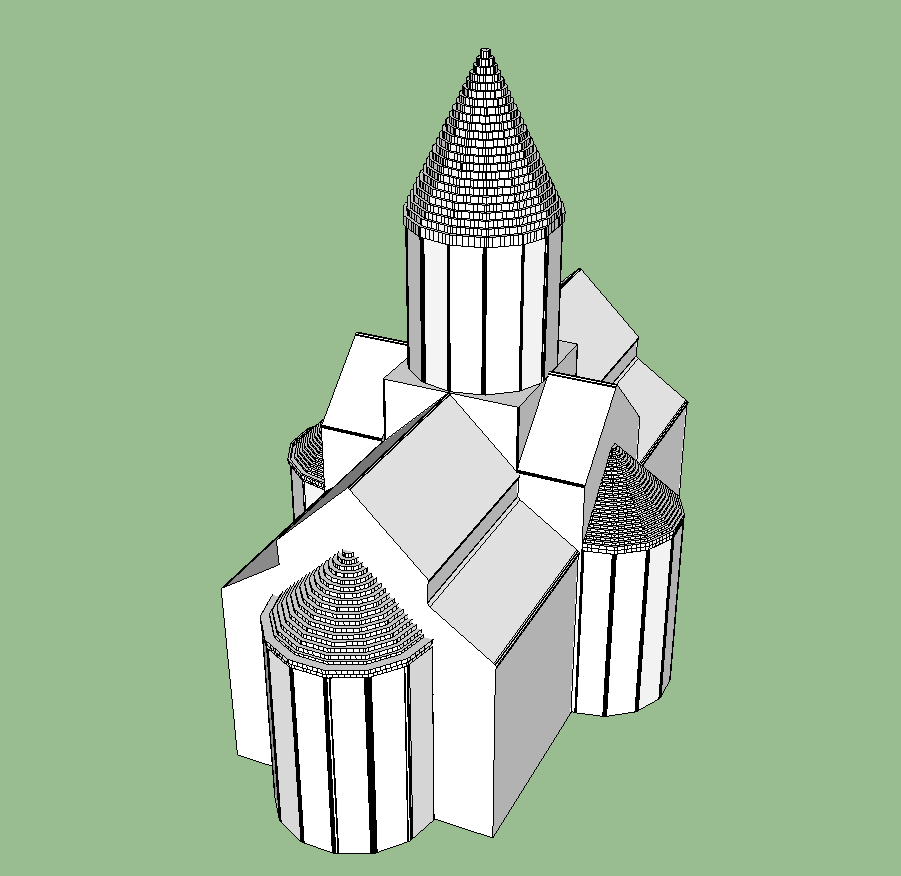
\includegraphics[width=0.18\textwidth]{spitak_11.png} \\
%(a) & (b) & (c) & (d) & (e)\\
% 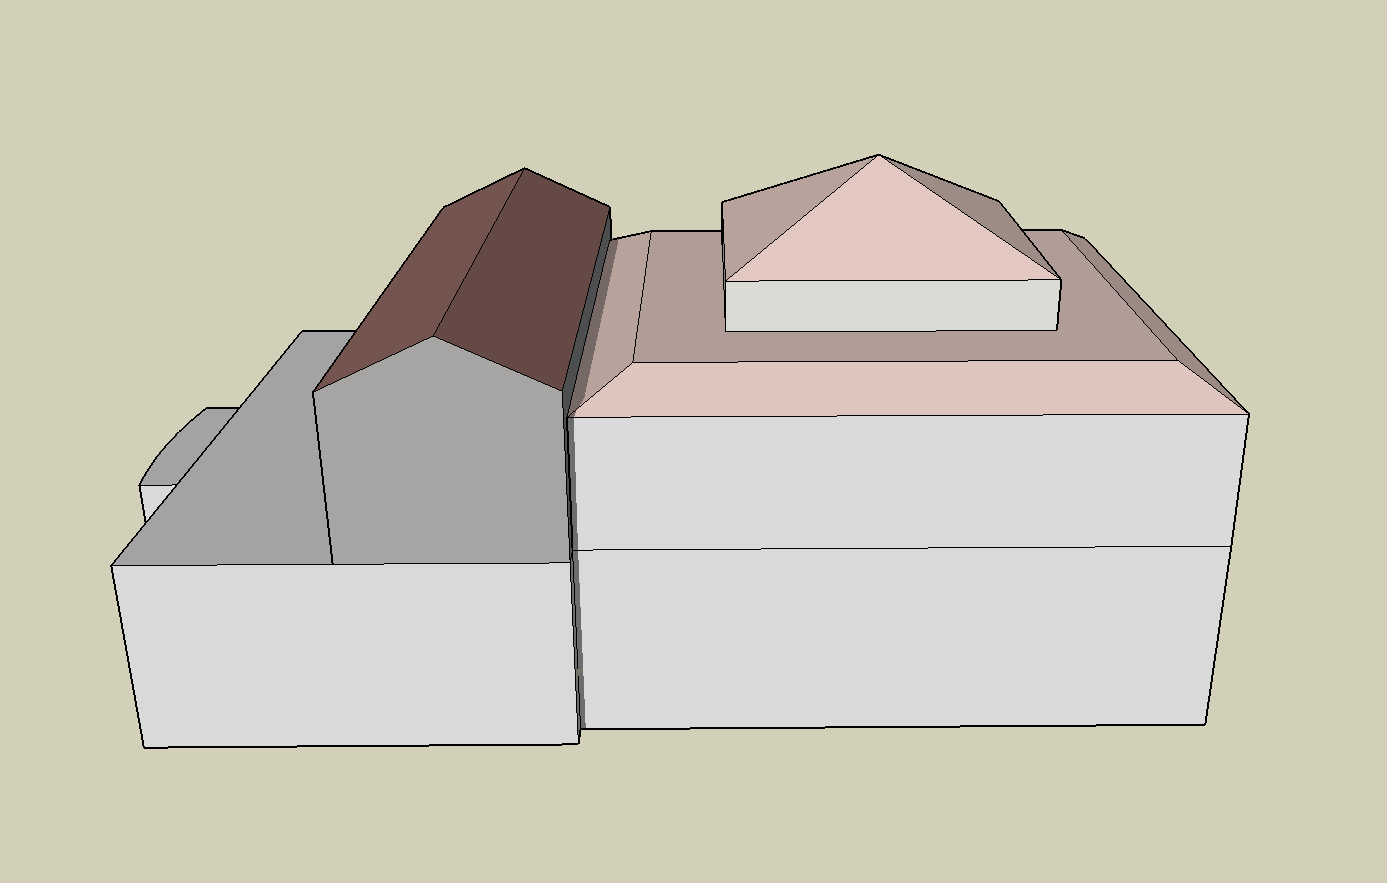
\includegraphics[width=0.18\textwidth]{doe_1.png} &
% 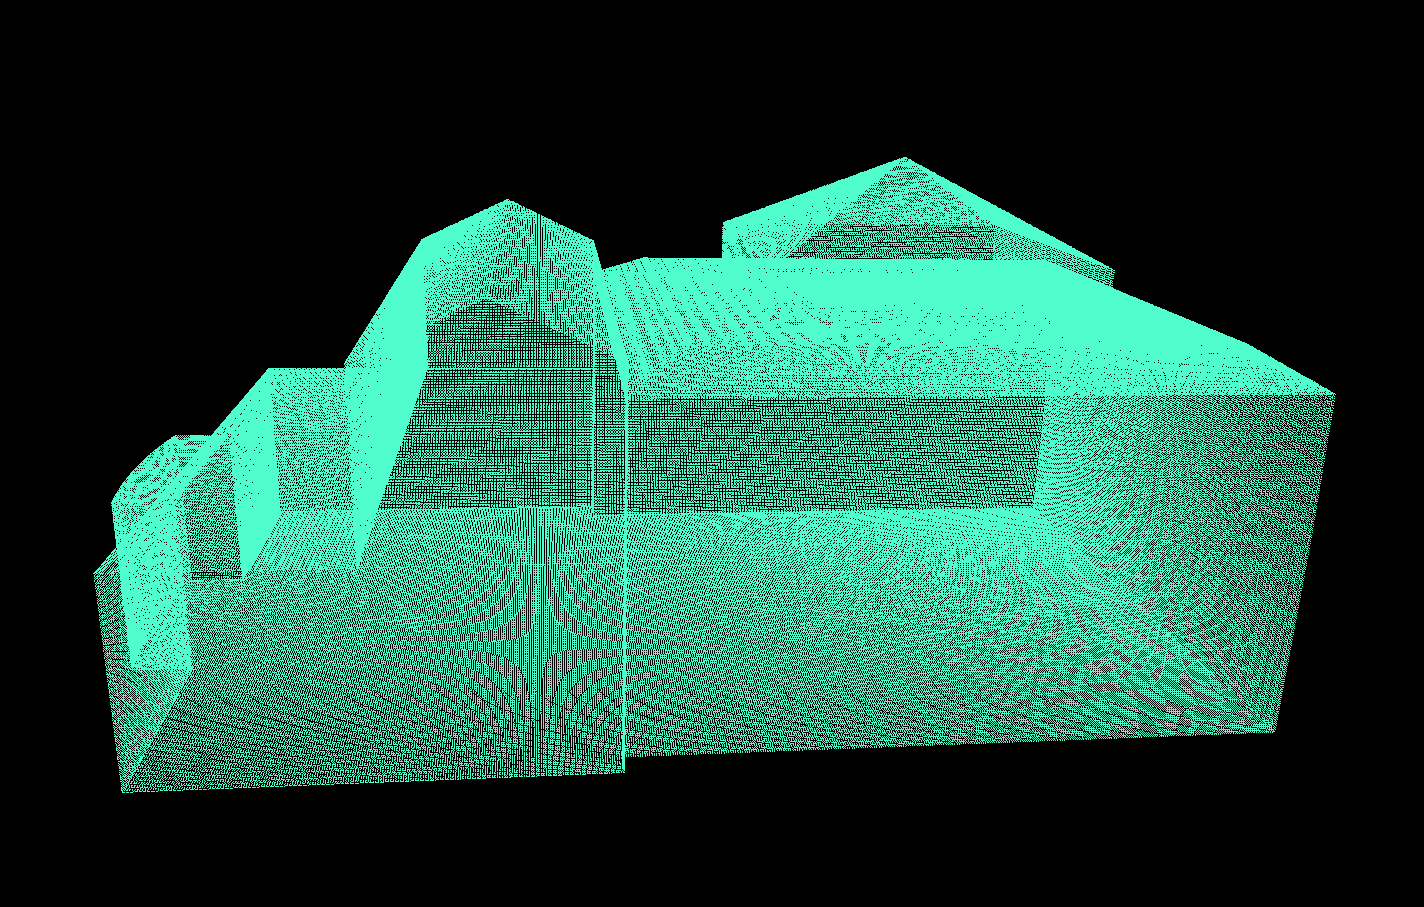
\includegraphics[width=0.18\textwidth]{doe_2.png} &
% 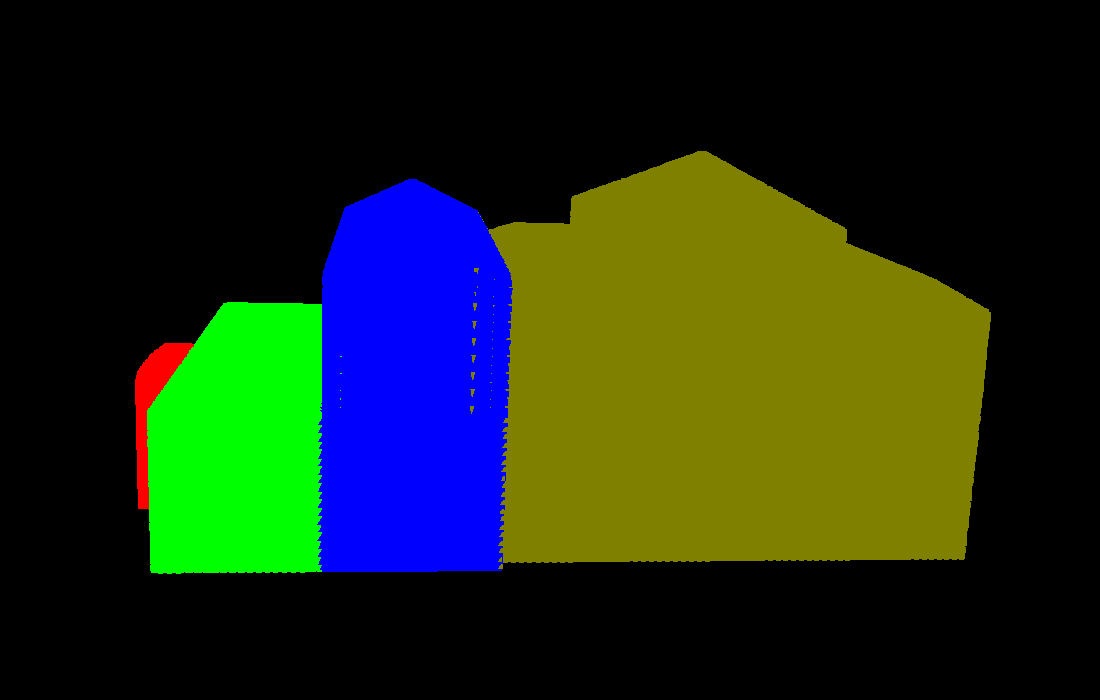
\includegraphics[width=0.18\textwidth]{doe_7.png} &
% 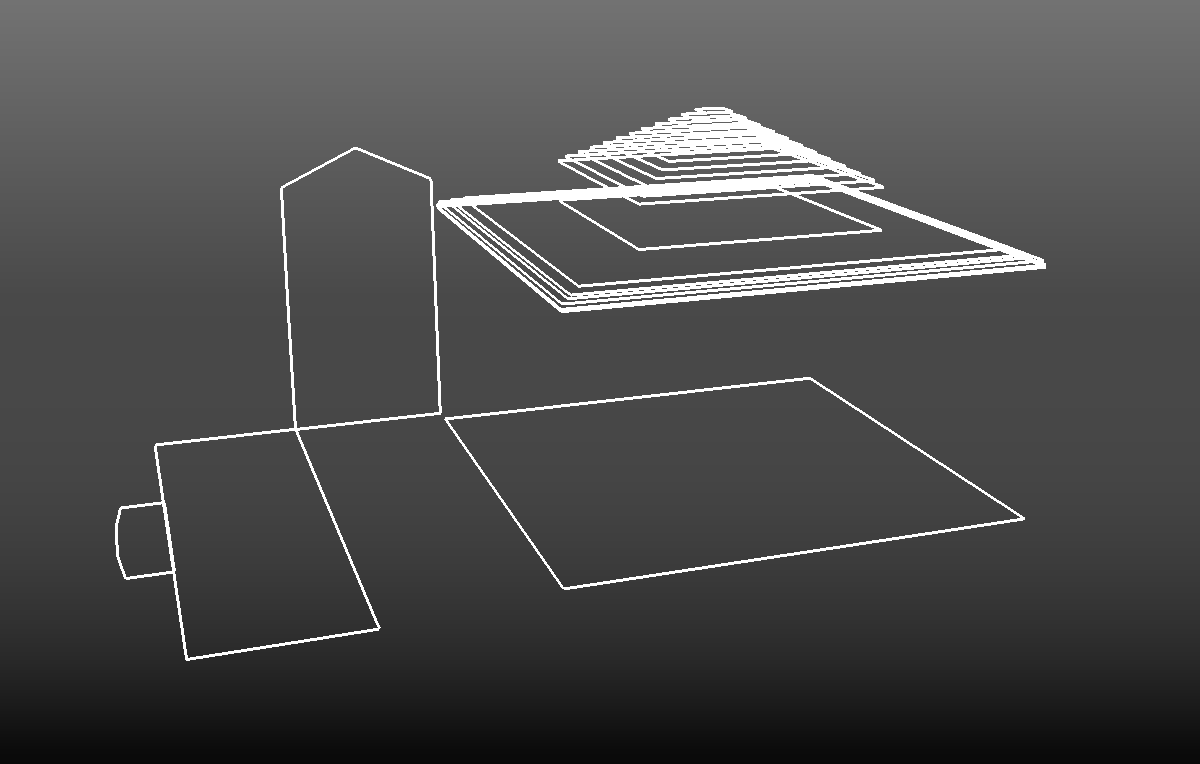
\includegraphics[width=0.18\textwidth]{doe_9.png} &
% 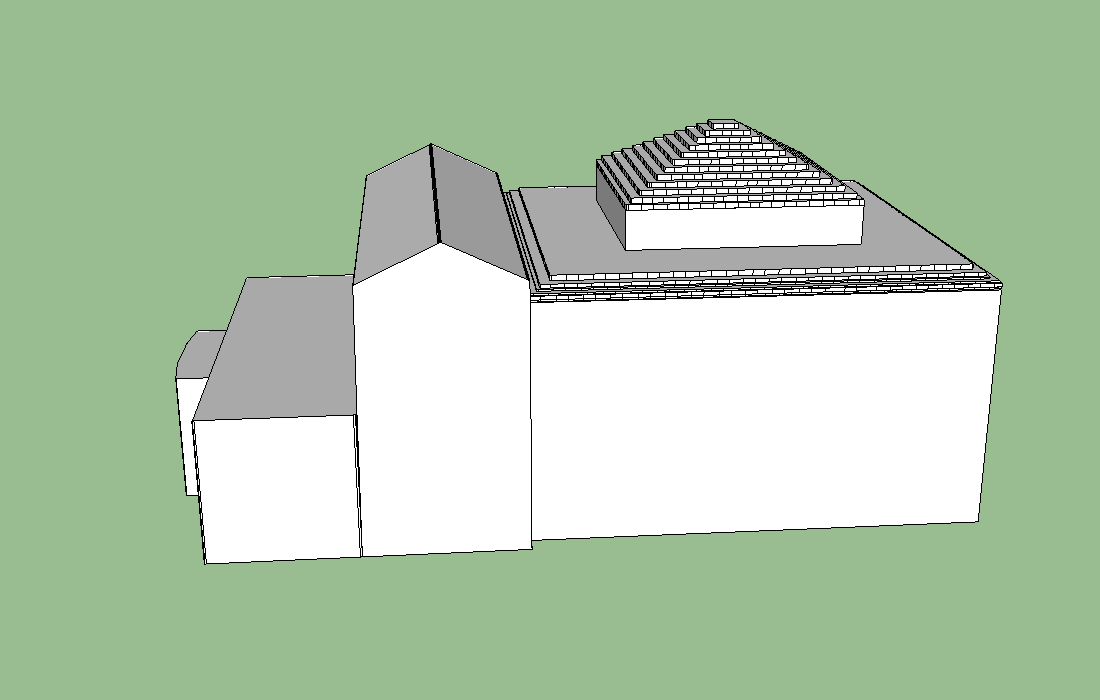
\includegraphics[width=0.18\textwidth]{doe_11.png} &
% 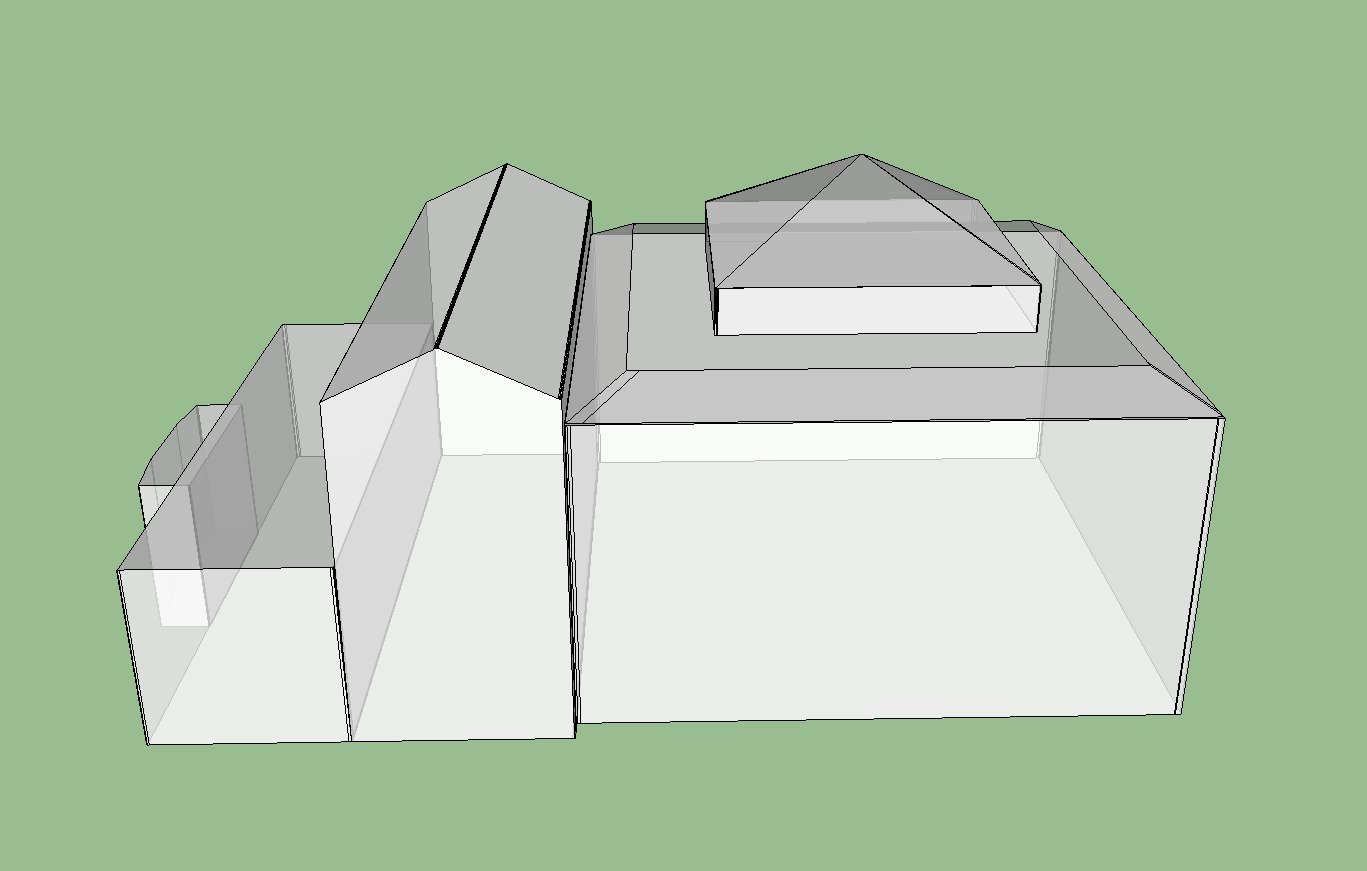
\includegraphics[width=0.18\textwidth]{doe_3.png} \\
% (a) & (b) & (c) & (d) & (e) & (f) \\
% 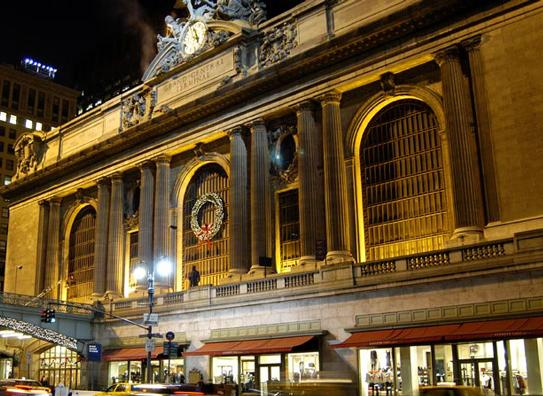
\includegraphics[width=0.18\textwidth]{GCT_1.jpg} &
% 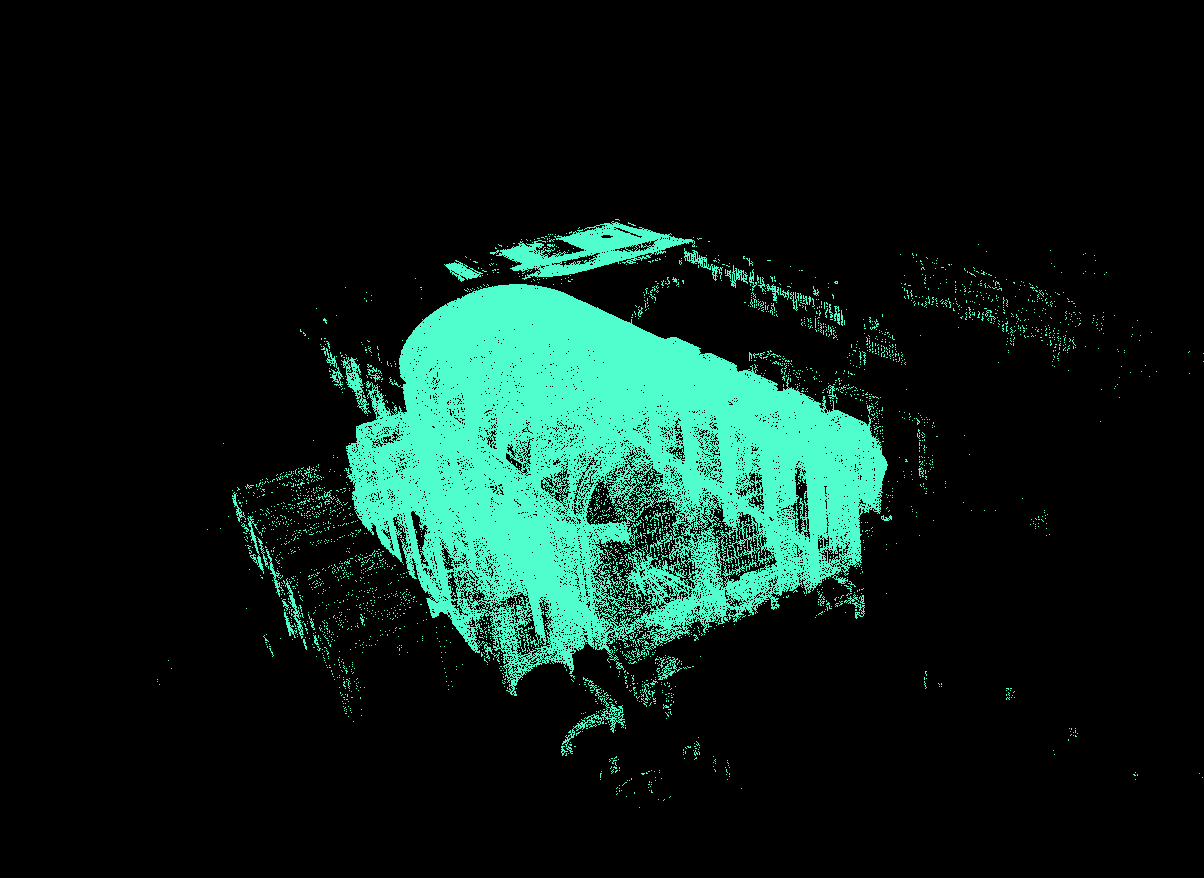
\includegraphics[width=0.18\textwidth]{GCT_2.png} &
% 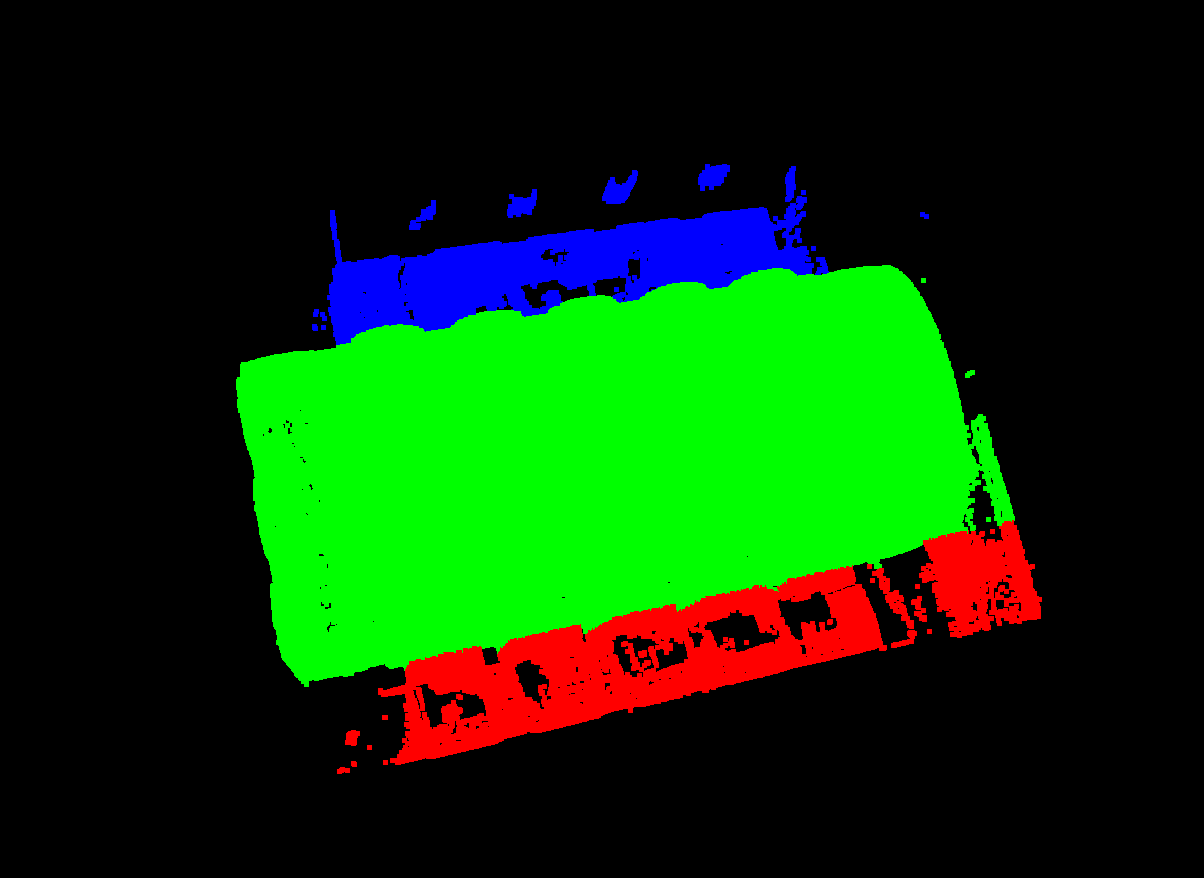
\includegraphics[width=0.18\textwidth]{GCT_7.png} &
% 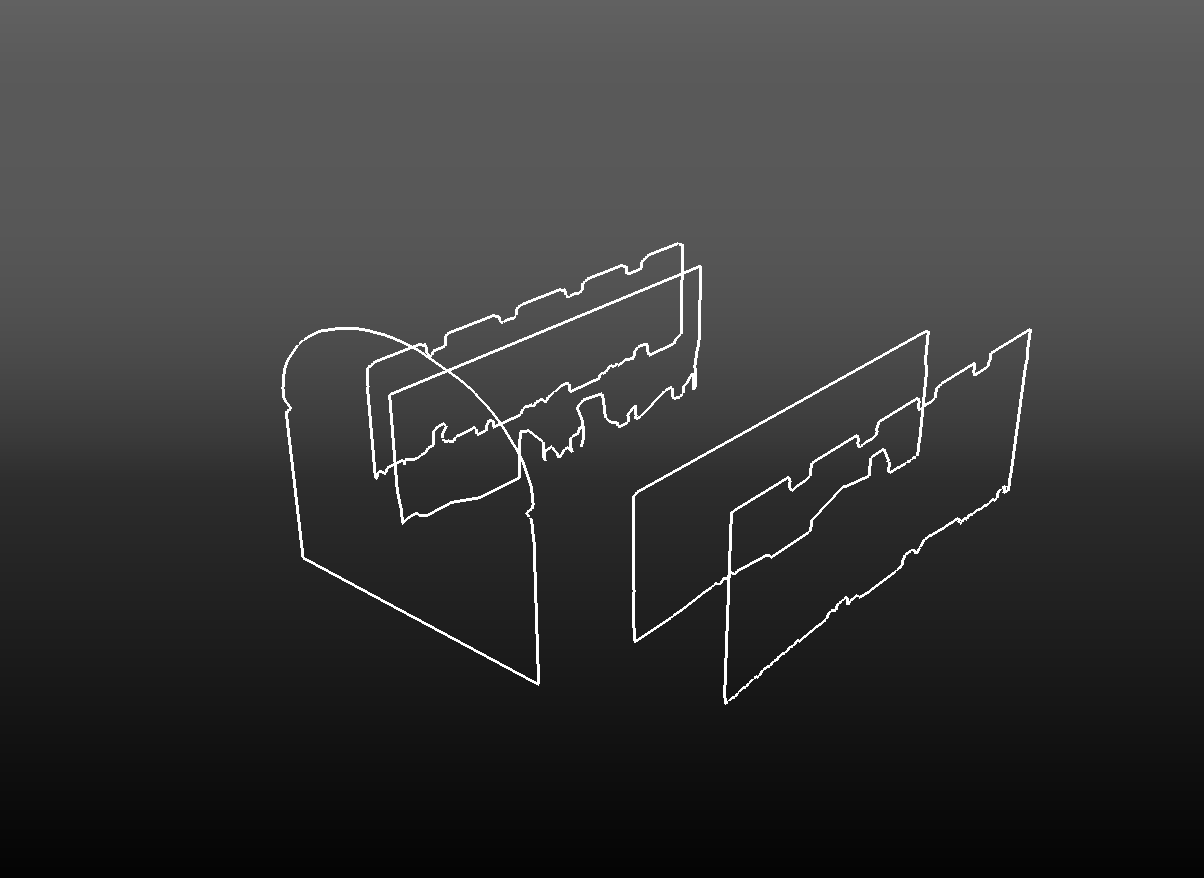
\includegraphics[width=0.18\textwidth]{GCT_9.png} &
% 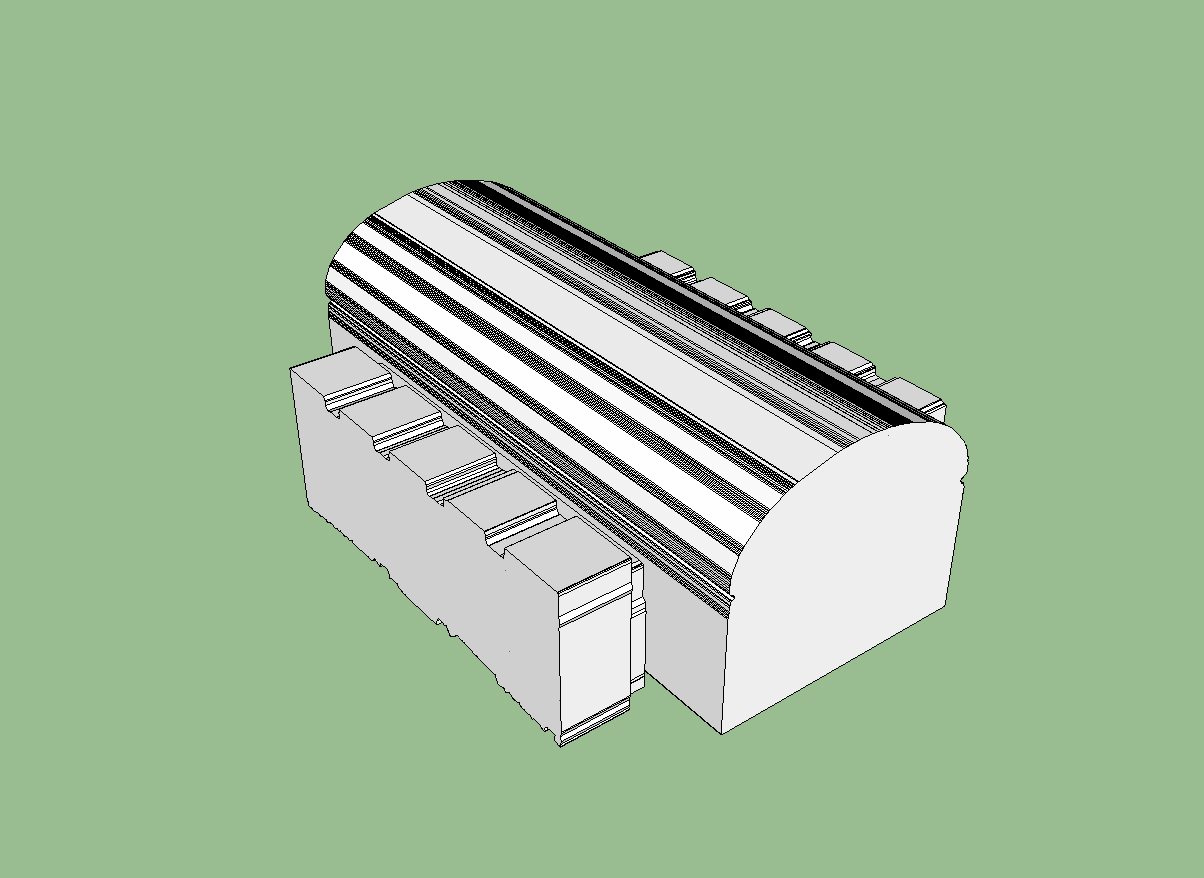
\includegraphics[width=0.18\textwidth]{GCT_10.png} \\
% (a) & (b) & (c) & (d) & (e) \\
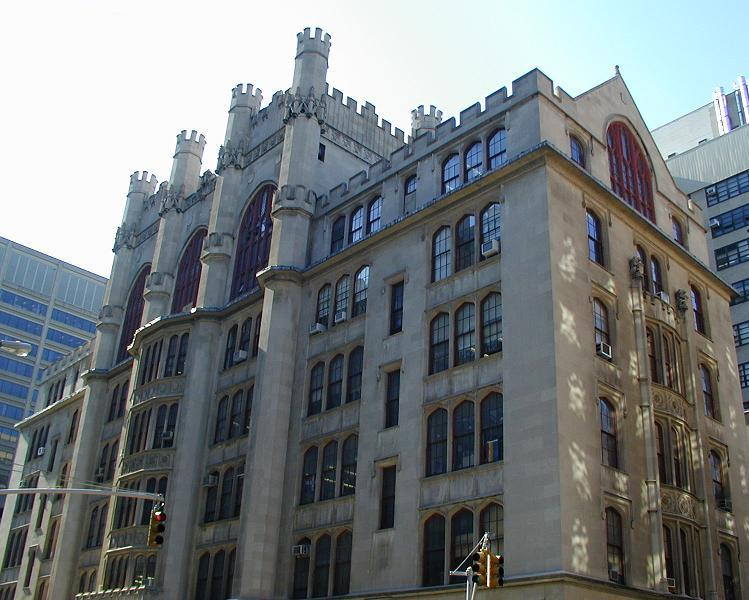
\includegraphics[width=0.18\textwidth]{HunterPhoto.jpg} &
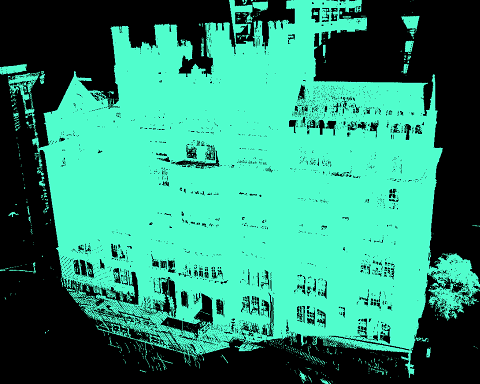
\includegraphics[width=0.18\textwidth]{point_cloud.png} &
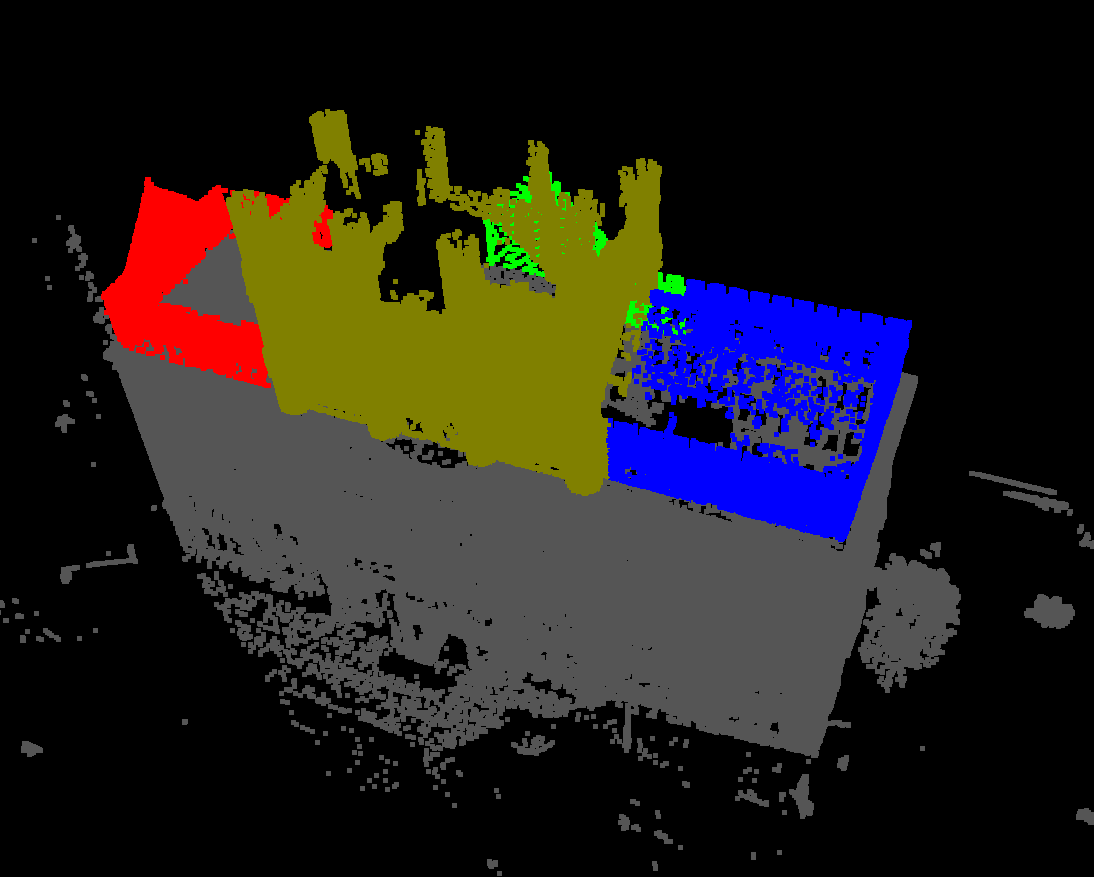
\includegraphics[width=0.18\textwidth]{TH_7.png} &
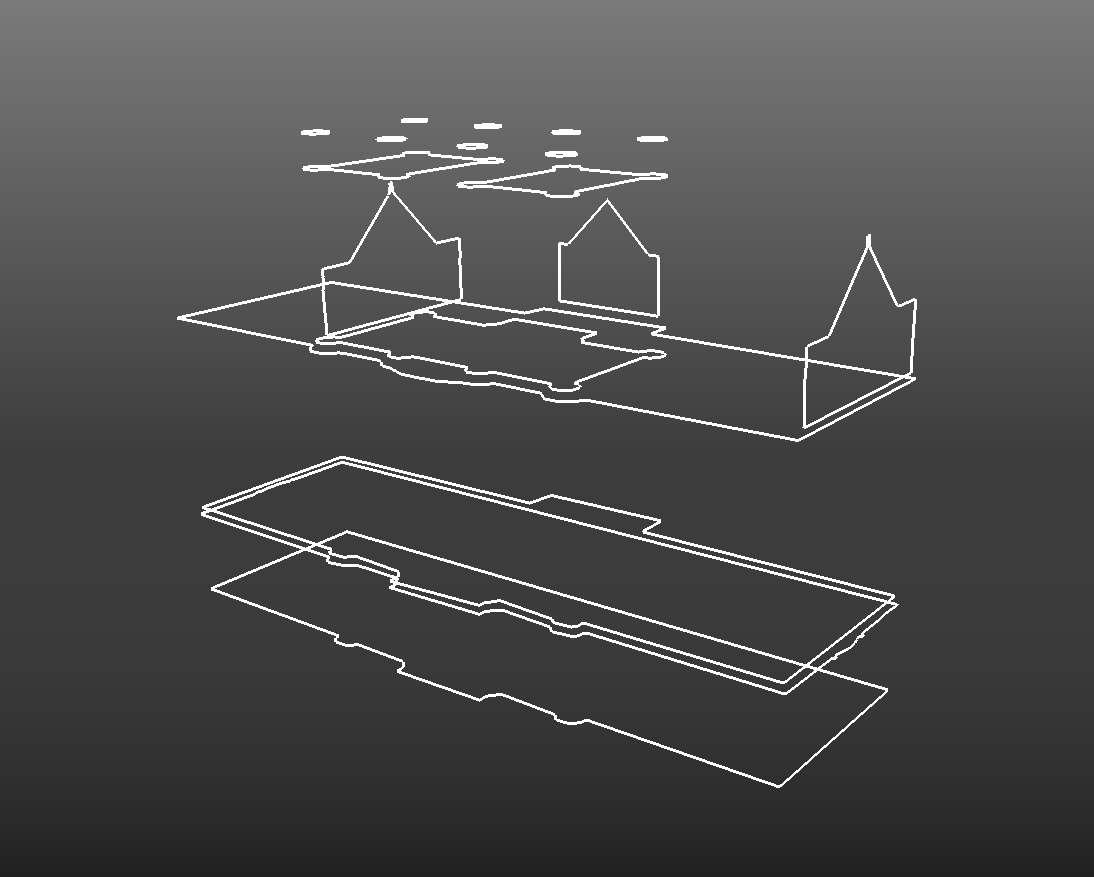
\includegraphics[width=0.18\textwidth]{TH_9.png} &
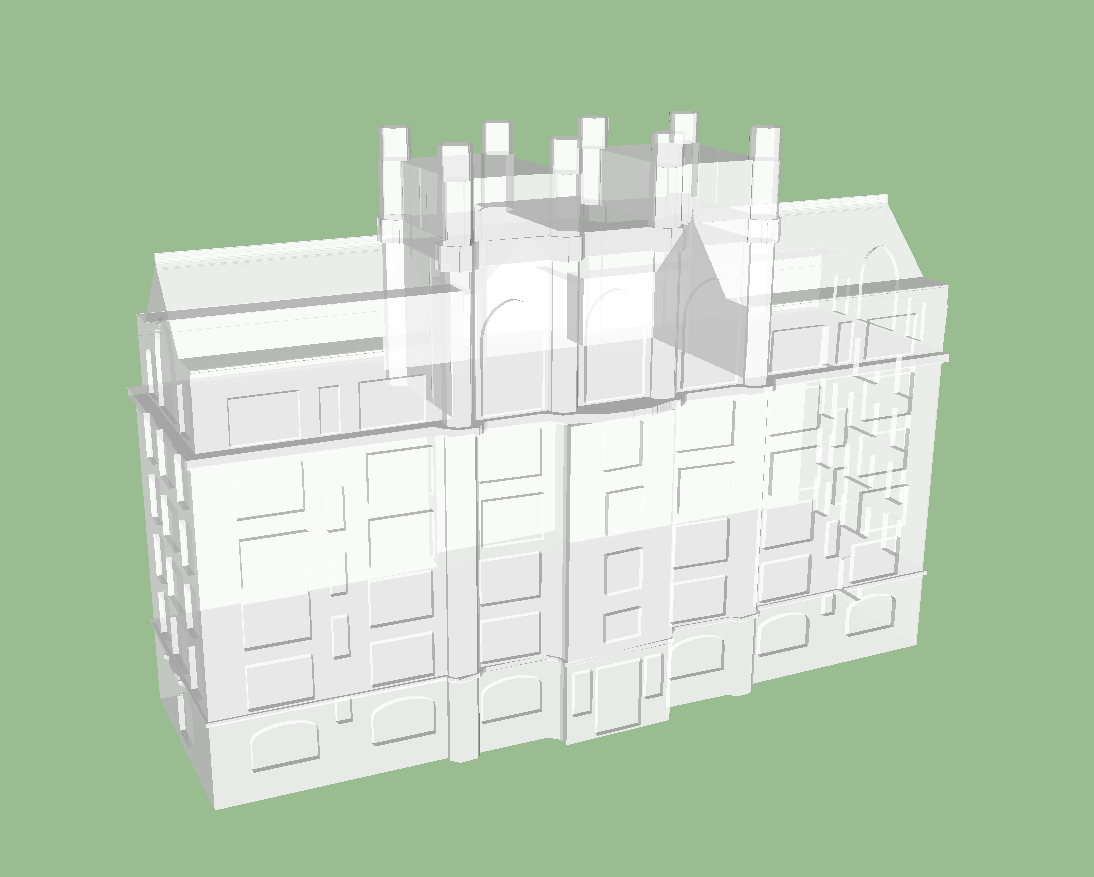
\includegraphics[width=0.18\textwidth]{TH_3.png} \\
%(a) & (b) & (c) & (d) & (e) \\
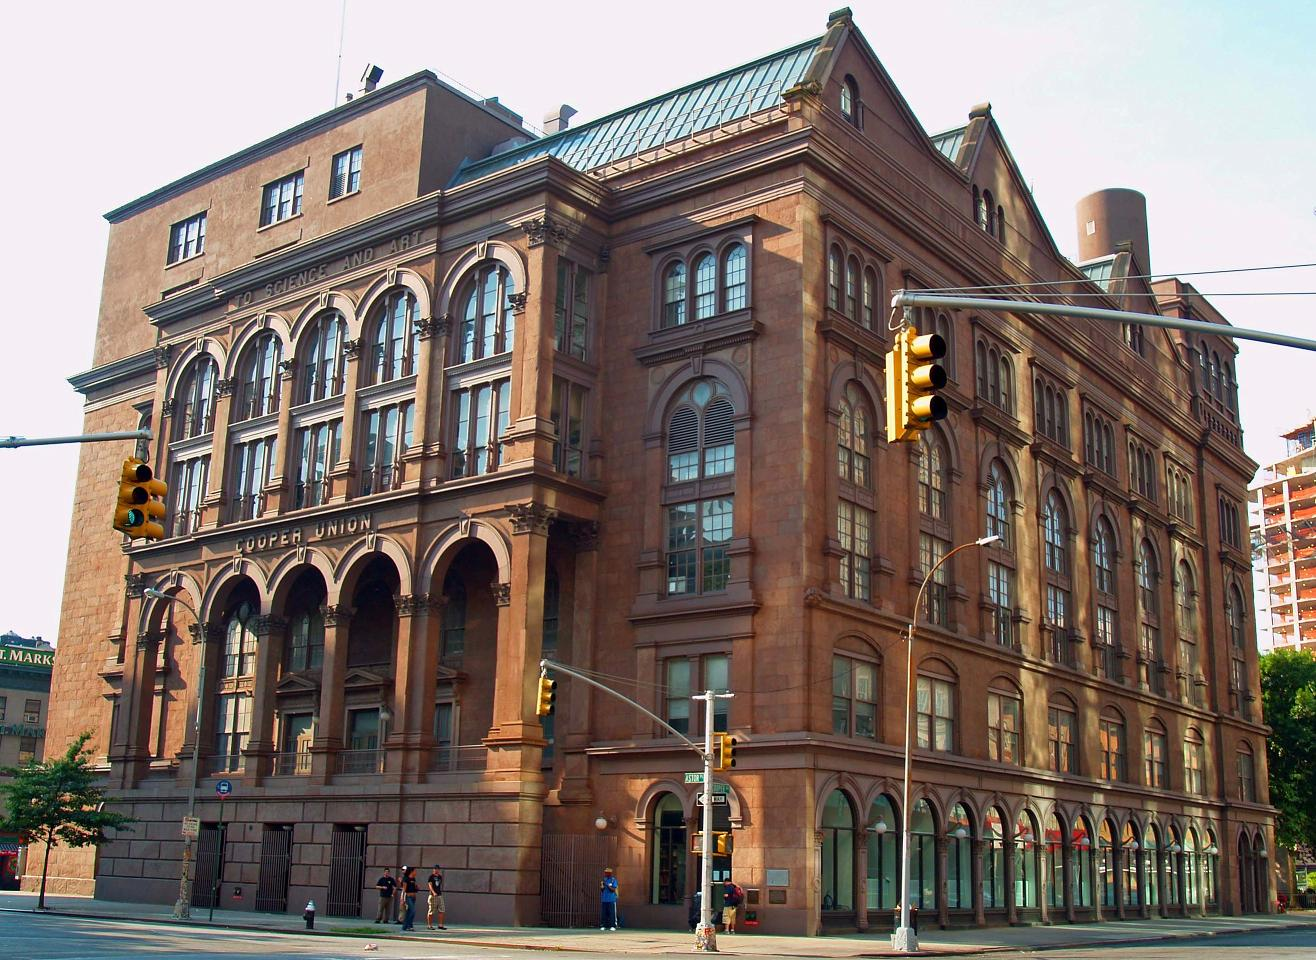
\includegraphics[width=0.18\textwidth]{real_cu_1.jpg} &
\includegraphics[width=0.18\textwidth]{real_cu_2.png} &
\includegraphics[width=0.18\textwidth]{real_cu_7.png} &
\includegraphics[width=0.18\textwidth]{real_cu_9.png} &
\includegraphics[width=0.18\textwidth]{real_cu_3.png} \\
% (a) & (b) & (c) & (d) & (e) \\
\includegraphics[width=0.18\textwidth]{opernhaus_1.png} &
\includegraphics[width=0.18\textwidth]{opernhaus_2.png} &
\includegraphics[width=0.18\textwidth]{opernhaus_3.png} &
\includegraphics[width=0.18\textwidth]{opernhaus_4.png} &
\includegraphics[width=0.18\textwidth]{opernhaus_6.png} \\
(a) & (b) & (c) & (d) & (e)
\end{tabular}
\end{center}
\caption{Experimental results.
(a) original model / picture,
(b) 3D point cloud of (a),
(c) segmentation,
(d) keyslices, and
(e) reconstructed model with windows.
The data of the Opernhaus Hannover in the bottom row is provided courtesy of 
the Institute of Cartography and Geoinformatics, University of Hannover.
}
\label{fig:results}
\end{figure*}

%\section{Performance Evaluation}
%
To measure the error of a reconstructed 3D model, we first transform it
to the 3D coordinate system.
The error $E$ is measured as the distance between the 3D points in the cloud
to their closest planes in the reconstructed model $M$:
\begin{equation}
E = \frac{1}{|X|}\sum_{x\in{X}}{d(x, M)}
\label{eq:em}
\end{equation}
where $X$ is the set of 3D points, and distance
$d(x, M) = \text{min}_{p \in M}\lVert x - p \lVert$ is the minimum
Euclidean distance from a 3D point $x$ to its closest face $p$ of $M$.

% \begin{figure} [htbp]
% \begin{center}
% \begin{tabular}{cc}
% \includegraphics[width=0.22\textwidth]{error_1000_32_4.png} &
% \includegraphics[width=0.22\textwidth]{error_1000_4_1.png} \\
% (a) & (b)
% \end{tabular}
% \end{center}
% \caption{The deviation map of the 3D point cloud.
% (a) The result with $\tau_r$ = 4 and $\tau_d$ = 32.
% (b) The result with $\tau_r$ = 1 and $\tau_d$ = 4. }
% \label{fig:EM}
% \end{figure}
%
% To visualize the error between real 3D data and the inferred model,
% we generate deviation map images.
% Two such images are shown in \Fig{EM} for the PCD in
% \Figb{IR_2_DXF}.
% The deviation maps are constructed as follows.
% For each face $p$ of $M$, a corresponding texture image is computed.
% The intensity of each pixel in the texture image is determined by the error
% of the corresponding 3D points computed by \Eq{em}.
% The accuracy of the reconstructed model is controlled by Hausdorff distance
% threshold $\tau_d$ and BPA refinement radius $\tau_r$.
% Threshold $\tau_d$ determines the accuracy of keyslice detection and $\tau_r$
% determines the accuracy of boundary vectorization.
%
\Tbl{em} lists the relationship among the $\tau_d$, errors,
number of faces, and model size for the input data in \Figb{IR_2_DXF}.
The unit for $\tau_d$ is in pixels and the unit for error is in meters.
The size of the original point cloud for the 3D building is more than 700 MB.
From the table, we can see that even for the most accurate model,
the size is dramatically reduced compared with the original 3D PCD.
This is a desirable property for web-based applications.
These models were generated on a laptop PC with an Intel Core 2 T7200 CPU 
at 2.0 GHz with 2.0 GB RAM.
Future work includes the optimization of the BPA vectorization module since
it consumes approximately 70\% of the computation time.

%\setlength{\tabcolsep}{4pt}
\begin{table}[hbtp]
\begin{center}
\begin{tabular}[t]{||c||c|c|c|c||}
\hline
$\tau_d $(pixel) & Error (m)& \# of faces & Size (KB) & time (s) \\ \hline \hline
64 & .658 $\pm$ .158 & 1471  & 15  & 1977 \\ \hline
32 & .294 $\pm$ .103 & 3284  & 32  & 2353 \\ \hline
16 & .141 $\pm$ .058 & 8574  & 86  & 3008 \\ \hline
8  & .131 $\pm$ .074 & 13955 & 137 & 3696 \\ \hline
4  & .094 $\pm$ .068 & 27214 & 261 & 5391 \\ \hline
2  & .088 $\pm$ .036 & 31331 & 335 & 7586 \\ \hline
1  & .083 $\pm$ .041 & 32187 & 337 & 10927\\ \hline
\end{tabular}
\end{center}
\caption{Error measurements for reconstruction of Thomas Hunter dataset using
distance measurement threshold $\tau_d$ and BPA radius threshold $\tau_r = 4$.}
\label{tbl:em}
\end{table}
%\setlength{\tabcolsep}{1.4pt}

\subsection{Model Comparison}

Although models generated by 3D BPA are of high resolution, they usually
require excessive storage capacity.
The model in \Fig{TH_BPA}, for example, needs almost 400 MB of storage,
which prevents this solution from being applied to web-based applications.
One way to improve matters is to apply some approximation/decimation
technique to reduce the space required by these models.

The holes in the 3D BPA model in \Fig{TH_BPA} are present in the
original dataset.
They are due to the fact that the laser never reflected back to
the scanner after penetrating the glass windows.
The 3D BPA method is deficient in filling these holes.
We counter this problem by first applying a symmetry-based hole filling
algorithm on the 2D slices to create enhanced slices that are processed
by an adaptive 2D BPA method to fill gaps.
Finally, an extrusion operation is applied to create a watertight 3D model.

\begin{figure}[htbp]
\begin{center}
\begin{tabular}{cc}
\includegraphics[width=0.22\textwidth]{BPA_TH.png} &
\includegraphics[width=0.22\textwidth]{BPA_TH_1.png}
\end{tabular}
\end{center}
\caption{Dense triangulated BPA mesh cropped from \Figb{IR_2_DXF}.}
\label{fig:TH_BPA}
\end{figure}

Among all mesh reduction techniques, {\it qslim} is one of the most
sophisticated and efficient algorithms \cite{BPA_GH}.
We carried out a comparison between models generated by our proposed
method and those approximated by {\it qslim}.
The comparisons were conducted on models sharing the same number of faces.
It is worth noting that {\it qslim} ran out of memory on the 3D model data
generated by BPA in \Fig{TH_BPA}.
In order to reduce the size of the model for {\it qslim} to work, we had
to either downsample the 3D model generated by BPA or split it into
sub-models which can be handled by {\it qslim}.

\begin{figure}[htbp]
\begin{center}
\begin{tabular}{cc}
\includegraphics[width=0.22\textwidth]{comp_32_2_qslim.png} &
\includegraphics[width=0.22\textwidth]{comp_4_2_qslim.png} \\
(a) & (b) \\
\includegraphics[width=0.22\textwidth]{comp_32_2.png} &
\includegraphics[width=0.22\textwidth]{comp_4_2.png} \\
(c) & (d)
\end{tabular}
\end{center}
\caption{
Models generated by {\it qslim} with (a) 2,000 and (b) 32,000 faces
and by our approach with (c) 2,000 and (d) 32,000 faces.}
\label{fig:TH_comp}
\end{figure}

\Figa{TH_comp} and \Figc{TH_comp} respectively depict the models generated
by {\it qslim} and our proposed method with approximately 2,000 faces each.
Higher resolution models with roughly 32,000 faces each are shown in
\Figb{TH_comp} and \Figd{TH_comp}.
Notice that the models approximated by {\it qslim} are inferior since they
do not preserve the sharpness of the original model and are replete with
holes. Our symmetry detector and extrusion operation guarantees no holes.

There have been recent attempts at preserving the sharp features of buildings
during the decimation process \cite{moser09}.
Nevertheless, the output model remains a triangulated mesh.
The benefit of our approach is that we represent the model with a set of
polygons and an associated grammar of extrusion/taper operations.
This furnishes a powerful mechanism by which to infer a procedural
model through 3D point clouds.

%%%%%%%%%%%%%%%%%%%%%%%%%%%%%%%%
%%%%%%   Conclusion and Future Work%%%
%%%%%%%%%%%%%%%%%%%%%%%%%%%%%%%%
\section{Conclusion}

This paper has presented an efficient algorithm for lightweight 3D modeling
of urban buildings from range data.
Our work is based on the observation that buildings can be viewed as the
combination of two basic operations: extrusion and taper.
The range data is partitioned into volumetric slabs whose 3D points are
projected onto a series of uniform cross-sectional planes.
The points in those planes are vectorized using an adaptive BPA algorithm
to form a set of polygonal contour slices.
Prominent keyslices are extracted from this set.
Applying extrusion to these keyslices forms lightweight 3D models.
We achieve further geometry compression by detecting a series of
slices that coincide with a linear tapering operation.

\begin{figure} [htbp]
\begin{center}
\begin{tabular}{cc}
\includegraphics[width=0.22\textwidth]{limitation_1.png} &
\includegraphics[width=0.22\textwidth]{limitation_2.png}
\end{tabular}
\end{center}
\caption{Examples of failed cases:
      (a) intersection of two extruded structures.
      (b) intersection of a tapered structure with an extruded structure.}
\label{fig:ER_Lmt}
\end{figure}

One limitation of the proposed method is that it could not handle the
intersection of two structures from different directions.
For example, \Figa{ER_Lmt} shows a case where two extruded structures
intersect and \Figb{ER_Lmt} shows one with intersection of a tapered
structure and an extruded structure.
Therefore, one future direction of our work is to expand our system to
handle them.
Additional future work is to investigate the modeling of the ``follow-me''
geometry structure.
This is a more complicated geometry structure featured in Google SketchUp
that exists when the model can be reconstructed by moving a cross-sectional
unit along a curve trajectory.
Finally, we will optimize the performance of the BPA vectorization module,
which consumes the bulk of the computation time.

\bibliographystyle{IEEEtran}
\bibliography{egbib}

\end{document}


